\documentclass[dvipsnames]{simplenote}    % Specifies the document style.
% \documentclass[dvipsnames]{cernatsnote}    % Specifies the document style.
\usepackage{amssymb}
\usepackage[T1]{fontenc}  % allows for \textsc and \textbf in one 
\usepackage{xstring}  % string manipulation
\usepackage[normalem]{ulem} % underlines
\usepackage{cite}
\usepackage{xfrac}

\listfiles  % writes current versions into log
% Contains user definitions %%%%%%%%%%%%%%%%%%%%%%%%%%%%%%%%%%%%%%%%%%%%%%%%%%%%%%%%%%%%%%%%%%%%%%%%%%%%%%%%%%%%%%%%%%%%%% 
\makeatletter
\newcommand{\inlineparagraph}{\@startsection{paragraph}{4}{\z@}%
  {-3.25ex \@plus -1ex \@minus -0.2ex}%
  {-1.2pt}%
  {}%
}

\newcommand{\noskipparagraph}{\@startsection{paragraph}{4}{\z@}%
  {-3.25ex \@plus -1ex \@minus -0.2ex}%
  {0.0001px}%
  {\scshape}%
}

\newcommand{\smallskipparagraph}{\@startsection{paragraph}{4}{\z@}%
  {-3.25ex \@plus -1ex \@minus -0.2ex}%
  {5px}%
  {\scshape}%
}
\makeatother

\newcommand{\ilparagraph}[1]{\inlineparagraph{\bfseries #1\textcolor{cern}{.}}}
% \newcommand{\myparagraph}[1]{\noskipparagraph{#1}}
% \newcommand{\myparagraph}[1]{\smallskipparagraph{\bfseries #1}}

% As the paragraphs don't have numbers, cref can't 
% refer to them. This makes cref use their name instead:
% \crefname{page}{page}{page}  % probably not needed
\crefformat{myparagraphlink}{#2\textsc{\textbf{#1}}#3}

\newcounter{myparagraphlink}
\makeatletter
\newcommand{\myparagraph}[1]{%
  \smallskipparagraph{\bfseries #1}%
  \refstepcounter{myparagraphlink}%
  \def\cref@currentlabel{[myparagraphlink][\arabic{myparagraphlink}][]#1}%
  \def\@currentlabelname{#1}%
}
\makeatother

% lengths
\newlength{\figurewidth}
\setlength{\figurewidth}{\linewidth}

\newlength{\subfigurewidth}
\setlength{\subfigurewidth}{0.5\textwidth}

% text arrangement
\newcommand{\tstack}[2]{$\substack{\text{\normalsize #1}\\\text{\tiny #2}}$} % stack two lines

% borders
\newcommand{\mytopmargin}[1]{\newgeometry{top=3cm}#1\restoregeometry}
\newcommand{\tinytopmargin}[1]{\newgeometry{top=1cm}#1\restoregeometry}

\newcommand{\tmpcapskip}[1]{
    \setlength{\abovecaptionskip}{5pt}
    \setlength{\belowcaptionskip}{5pt}
    #1
    \setlength{\abovecaptionskip}{10pt}
    \setlength{\belowcaptionskip}{0pt}
}



% Flowcharts
\usetikzlibrary{arrows, shapes, calc, positioning}
\tikzstyle{base} = [text=white, text centered, minimum width=1em, minimum height=1em]
\tikzstyle{startstop} = [base, ellipse, fill=CernRed!90, draw=CernRed!200]
\tikzstyle{io} = [base, trapezium, trapezium left angle=70, trapezium right angle=110, fill=CernNiceBlue, draw=CernBlue!200]
\tikzstyle{process} = [base, rectangle, rounded corners, fill=AtlasOrange!90, draw=AtlasOrange!200]
% \tikzstyle{process} = [base, rectangle, rounded corners, fill=CernYellow!90, draw=CernYellow!200]
\tikzstyle{test} = [base, signal, signal to=east and west, fill=GreenBellPepper!90, draw=GreenBellPepper!200]
% \tikzstyle{test} = [base, signal, signal to=east and west, fill=CernLightGreen!90, draw=CernLightGreen!200]
\tikzstyle{arrow} = [->, >=latex]

% Other
\newcommand\drawRect[5]{%
    \def\top{#1}
    \def\left{#2}
    \def\right{#3}
    \def\bottom{#4}
    \begin{tikzpicture}[remember picture, overlay]
        \draw[#5, thick] (\left,\top) -- (\right,\top) -- (\right,\bottom) -- (\left,\bottom) -- cycle;    
    \end{tikzpicture}
}

% Own commands and environments ---

% labels


% shortcuts
\newcommand{\ttt}[1]{\texttt{#1}}

\newcommand{\todo}[1]{{\color[RGB]{190, 130, 130} \textbf{TODO }\textit{#1}}}
\newcommand{\bone}{\textcolor{blue}{Beam 1}}
\newcommand{\btwo}{\textcolor{red}{Beam 2}}
\newcommand{\tcern}[1]{\textcolor{cern}{#1}}
\newcommand{\bfcern}[1]{\tcern{\bf#1}}
\newcommand{\beamone}{\textcolor{blue}{Beam 1}}
\newcommand{\beamtwo}{\textcolor{red}{Beam 2}}

\newcommand{\pro}[1]{\\\hspace{1em}{\color{GreenBellPepper}\textbf{+} #1}}
\newcommand{\con}[1]{\\\hspace{1em}{\color{CernRed}\hspace{.1em}\textbf{--}\hspace{.2em} #1}}
\newcommand{\sep}{\\\hspace{1em}{- - -}}

\newcommand{\textAD}[2]{$\partial$Q$_{#1}$/$\partial$2J$_{#2}$}

% maths



\newcommand{\of}[1]{\left(#1\right)}    % 'function of', i.e. (x) with proper parenthesis
\newcommand{\ReOf}[1]{\Re\left[#1\right]}    % 'function of', i.e. (x) with proper parenthesis
\newcommand{\ImOf}[1]{\Im\left[#1\right]}    % 'function of', i.e. (x) with proper parenthesis
\newcommand{\E}[1]{\cdot 10^{#1}}

\newcommand{\fof}[1]{\left(#1\right)}

\newcommand{\overeq}[1]{\overset{\mathmakebox[\widthof{=}]{#1}}{=}}
\newcommand{\myover}[2]{\overset{\mathmakebox[\widthof{$#2$}]{#1}}{#2}}
\newcommand{\myunder}[2]{\underset{\mathmakebox[\widthof{$#2$}]{#1}}{#2}}
\newcommand{\myoverunder}[3]{\overset{\mathmakebox[\widthof{$#2$}]{#1}}{\underset{\mathmakebox[\widthof{$#2$}]{#3}}{#2}}}

% Environments

\newenvironment{wider}[1][10pt]{
    \begin{columns}
        \column{\dimexpr\paperwidth-#1}
    }{
      \end{columns}%
}

\newlist{mytemize}{itemize}{1}
\setlist[mytemize,1]{topsep=2pt, itemsep=-0.5ex, partopsep=1ex, parsep=1ex, label=\smallbullet, rightmargin=\leftmargin}


\newcommand{\textimportant}[1]{\textbf{\textsc{#1}}}
\newlist{important}{description}{1}
\setlist[important,1]{itemindent=-10pt, leftmargin=10pt-\itemindent, parsep=2pt, font=\textimportant, rightmargin=\leftmargin}


% Underlines https://tex.stackexchange.com/a/27260/213738
\newcommand{\udot}[1]{%
    \tikz[baseline=(todotted.base)]{
        \node[inner sep=1pt,outer sep=0pt] (todotted) {#1};
        \draw[dotted] (todotted.south west) -- (todotted.south east);
    }%
}%

\newcommand{\udensdot}[1]{%
    \tikz[baseline=(todotted.base)]{
        \node[inner sep=1pt,outer sep=0pt] (todotted) {#1};
        \draw[densely dotted] (todotted.south west) -- (todotted.south east);
    }%
}%

\newcommand{\uloosdot}[1]{%
    \tikz[baseline=(todotted.base)]{
        \node[inner sep=1pt,outer sep=0pt] (todotted) {#1};
        \draw[loosely dotted] (todotted.south west) -- (todotted.south east);
    }%
}%

\newcommand{\udash}[1]{%
    \tikz[baseline=(todotted.base)]{
        \node[inner sep=1pt,outer sep=0pt] (todotted) {#1};
        \draw[dashed] (todotted.south west) -- (todotted.south east);
    }%
}%

\newcommand{\udensdash}[1]{%
    \tikz[baseline=(todotted.base)]{
        \node[inner sep=1pt,outer sep=0pt] (todotted) {#1};
        \draw[densely dashed] (todotted.south west) -- (todotted.south east);
    }%
}%

\newcommand{\uloosdash}[1]{%
    \tikz[baseline=(todotted.base)]{
        \node[inner sep=1pt,outer sep=0pt] (todotted) {#1};
        \draw[loosely dashed] (todotted.south west) -- (todotted.south east);
    }%
}%


% Create linkable options
\newcommand{\raisedtaget}[1]{\raisebox{\ht\strutbox}{\hypertarget{#1}{}}}

% replace \_ with _ and assign to \temp.
% this way options with underscores can be used
\newcommand{\subforlink}[1]{%
  \saveexpandmode\noexpandarg
  \StrSubstitute{#1}{\_}{_}[\tttemp]%
  \StrSubstitute{\tttemp}{-}{_}[\temp]%
  \restoreexpandmode
}

% make all options linkable via \opt command below. raisebox is needed, as target is at the base of the line
\newcommand{\defopt}[1]{\subforlink{#1}\raisebox{\ht\strutbox}{\hypertarget{\temp}{}}\texttt{#1}}
\newcommand{\opttarget}[2]{\subforlink{#1}\hypersetup{hidelinks}{\hyperlink{\temp}{\dashuline{#2}}}}
\newcommand{\opt}[1]{\opttarget{#1}{\texttt{#1}}}
\newcommand{\textttu}[1]{\defopt{#1}\texttt{:}}
\newlist{options}{description}{1}
\setlist[options,1]{itemindent=-20pt, leftmargin=20pt-\itemindent, parsep=2pt, font=\textttu, rightmargin=\leftmargin}
% \newlist{options}{itemize}{1}
% \setlist[options,1]{itemindent=0pt, leftmargin=80pt, parsep=2pt, font=\texttt}

% \newcommand{\subdescriptionitem}[1]{\normalfont\textit{#1:}}
\newcommand{\subdescriptionitem}[1]{\textcolor{gray}{\textsc{\small #1}}}
\setlist[description,2]{itemindent=-20pt, leftmargin=-\itemindent, parsep=2pt, font=\subdescriptionitem, rightmargin=\leftmargin}
 
\newcommand{\subtestlistitem}[1]{\textcolor{gray}{\text{\small #1}}}
\newlist{testlist}{description}{2}
\setlist[testlist,1]{itemindent=-10pt, leftmargin=10pt-\itemindent, parsep=2pt, font=\textimportant, rightmargin=\leftmargin}
\setlist[testlist,2]{itemindent=-20pt, leftmargin=-\itemindent, parsep=2pt, font=\subtestlistitem, rightmargin=\leftmargin}


% \setlength{\abovecaptionskip}{-5em}
% \setlength{\belowcaptionskip}{-5em}


% Meta-Data %%%%%%%%%%%%%%%%%%%%%%%%%%%%%%%%%%%%%%%%%%%%%%%%%%%%%%%%%%%%%%%%%%%%%%%%%%%%%%%%%%%%%%% 

% \documentlabel{CERN-ACC-NOTE-2022-???}
\documentversion{Version 1.0}
\date{18.01.2023}
\title{A flexible nonlinear Resonance Driving Term based Correction Algorithm with feed-down}
\author{J. Dilly, R. Tom\'as}

% logbook: 
% Document Begin %%%%%%%%%%%%%%%%%%%%%%%%%%%%%%%%%%%%%%%%%%%%%%%%%%%%%%%%%%%%%%%%%%%%%%%%%%%%%%%%%% 

\keywords{nonlinear correction, insertion region, feed-down, LHC, HL-LHC, HiLumi}

\begin{document}
\graphicspath{
    {./images/}
    %{./images/}
}
\maketitle 

\begin{abstract}
The optics in the insertion regions around the interaction points of the LHC, and its upgrade project the High Luminosity LHC, 
are very sensitive to local magnetic errors due to the extremely high beta-functions present.
Local corrections need to take both beams into account, due to the common aperture of the magnets in these regions.
In collision optics, the non-zero closed orbit around the interaction point leads to a ``feed-down'' of high-order errors to lower orders, 
causing additional effects detrimental to beam lifetime. 
An extension to the proven method~\cite{BruningDynamicApertureStudies2004} for correcting these errors by locally suppressing resonance driving terms has been undertaken, 
not only taking this feed-down into account, but also adding the possibility of utilizing it such that the powering of higher-order correctors will compensate 
for lower order errors.
The existing correction scheme has also operated on the assumption of symmetric beta-functions of the optics in the two rings.
As this assumption can fail for a multitude of reasons, such as inherently asymmetric optics, 
an extension of this correction scheme has been developed removing the need for symmetry by operating on the two separate optics of the beams at the same time.
In contrast to earlier implementations, the target resonance driving terms to be corrected can also be flexibly changed. 
The mathematical background as well as the implementation of this new extension are presented in this note.
\end{abstract}


\tableofcontents
\newpage

% Motivation %%%%%%%%%%%%%%%%%%%%%%%%%%%%%%%%%%%%%%%%%%%%%%%%%%%%%%%%%%%%%%%%%%%%%%%%%%%%%%%%%%%%%%%

\section{Motivation}

% General Correction in the IRs ---

The sensitivity of accelerator beam optics to magnetic errors depends directly on the $\beta$-function, 
which is highest in the Insertion Regions (IR) around the Interaction Points (IP) 
with the lowest $\beta^*$ (the value of the $\beta$-function at the location of the IP).

Hence, studies of the possibility of correcting the non-linear magnetic errors in these regions in the Large Hadron Collider (LHC)
have already been of significant importance during its design phase:
It was envisaged to make use of the magnetic measurement data of the LHC 
magnets~\cite{SammutMathematicalFormulationPredict2006,SammutMathematicalFormulationPredict2007,SammutMathematicalFormulationPredict2009} to
simulate the machine in MAD-X~\cite{DeniauMADXUserGuide} and calculate the corrections to be used in the
machine~\cite{BruningFieldQualityIssues2004,BruningDynamicApertureStudies2004,TomasNonlinearCorrectionSchemes2009}.
While these simulation-based corrections produced great results in the arcs~\cite{PerssonChromaticCouplingCorrection2013}
in the IRs discrepancies with corrections from beam-based measurements
were observed~\cite{MacleanFirstMeasurementCorrection2015}.
The sources for these discrepancies are still not fully known.
Apart from the successful arc-corrections, 
simulations have nevertheless been a useful tool for the estimation of linear and non-linear 
effects in the IRs~\cite{MacleanNewApproachLHC2019,MacleanFirstMeasurementCorrection2015,
TomasCERNLargeHadron2010,DillyAmplitudeDetuningMisaligned2020}.
Magnetic-measurement based simulations have since supported 
the continuing endeavour to optimize the LHC machine performance
with beam-based corrections in the IRs~\cite{MacleanCommissioningNonlinearOptics2016,
MacleanNewMethodsMeasurement2017,MacleanNewLHCOptics2017,MacleanDetailedReviewLHC2019,
MacleanNewApproachLHC2019,MacleanProspectsBeambasedStudy2022},
and continue to be an invaluable tool in studying future machine layouts,
e.g. the installation of stronger magnets in the IR and the decrease of $\beta^*$ in operation in the High Luminosity upgrade of the 
LHC~(HL-LHC)~\cite{FartoukhHLLHCAcceleratorPhysics2015,BejarAlonsoHighLuminosityLargeHadron2020},
which is foreseen to result in even tighter constraints on residual errors. 

At the same time the crossing-angle scheme of the collision optics creates large orbit bumps in the IRs,
leading to feed-down effects, the influence of which have been observed and investigated in the LHC.
For both, LHC and HL-LHC the need for corrections of this feed-down has been established
~\cite{MacleanNewMethodsMeasurement2017,
MacleanDetailedReviewLHC2019, 
MacleanNewApproachLHC2019,
MacleanProspectsBeambasedStudy2022,
MacleanFirstMeasurementCorrection2015,
MacleanNonlinearOpticsCommissioning2016,
MacleanLHCMD21712018, 
BuffatOpticsMeasurementCorrection2022}.

% Introduction of correction scheme ---

To estimate the powering of the corrector magnets, a local correction scheme
based on the Resonance Driving Terms (RDTs) in the IRs has been 
utilized~\cite{BruningDynamicApertureStudies2004}. 
Up to now, the implementation of this scheme calculated the correction based on a single input optics, 
for either Beam~1 or Beam~2, and made use of symmetries between the beams to optimize the correction for both beams. 
Cases will occur in which this symmetry does not hold, e.g. through the introduction of feed-down, or the use of inherently asymmetric optics.
An example for the latter is the flat optics~\cite{FartoukhAchromaticTelescopicSqueezing2013,FartoukhFlatTelescopicOptics2018},
in which $\beta^*$ in the two transversal planes no longer has identical values. 
These optics allow for a more distributed radiation deposition in the LHC magnets as well as an increase 
in luminosity~\cite{FartoukhFlatTelescopicOptics2018}.
Their feasibility has been studied during machine developments in the LHC~\cite{FartoukhFirstHighIntensityBeam2019}
and preliminary analysis regarding their influence on corrections and amplitude detuning has been conducted~\cite{DillyCorrectionAmpDet2018}.
A new and flexible version of the correction principle has been implemented~\cite{OMC-TeamIRNLRDTCorrection}, 
taking up to two optics into account and hence not relying on symmetry assumptions, allowing to target RDTs freely,
as well as including feed-down into the calculations. 
The implementation allows for the feed-down from higher orders to the RDT to be corrected, 
as well as using the feed-down from higher order corrector magnets to correct for lower order errors.
Theoretical background and the implementation details of this algorithm are presented in this report.

% The new correction script has since been used for extensive tracking studies, 
% investigating the influence of feed-down~\cite{DillyCorrectionsFeedDownNonLinear2021},
%  the correctability of asymmetric optics~\cite{DillyCorrectionsAsymmetricNonLinear2021}
% and the feasibility to correct systematic normal decapole errors in the separation and 
% recombination dipoles of the HL-LHC~\cite{DillyFeasibilityCorrectingSystematic2021,DillyCorrenctionsSystematicNormal2022}.
% Further studies are still ongoing and will be published in the near future.


% Mathematical Description %%%%%%%%%%%%%%%%%%%%%%%%%%%%%%%%%%%%%%%%%%%%%%%%%%%%%%%%%%%%%%%%%%%%%%%%%%%%%% 
\FloatBarrier
\section{Background}

\subsection{Nonlinear Correctors}

Due to the high $\beta$-functions around the experimental IPs, 
the optics of the LHC and HL-LHC are very sensitive to field imperfections in the surrounding triplets.
To compensate for these errors locally, both sides of the LHC IRs hosting experiments 
(ATLAS in IR1, ALICE in IR2, CMS in IR5 and LHCb in IR8) are equipped with linear and non-linear corrector packages.
As shown in the schematics of \cref{fig:irregionlhc,fig:irregionhllhc}, 
these packages are located within the common aperture region of the machines, between Q3 and the separation dipoles D1,
and hence contain common magnets for the two beams. 
Any correction should therefore take the optics of both beams into account.

In the experimental IRs of the LHC and in HL-LHC IR2 and IR8, nonlinear correctors for
skew and normal sextupoles ($a_3, b_3$), skew and normal octupoles ($a_4, b_4$) 
and normal dodecapoles ($b_6$) are available.
In IR1 and IR5 in the HL-LHC on the other hand, the corrector package will be upgraded to 
also include skew and normal decapoles ($a_5, b_5$) as well as skew dodecapoles ($a_6$)
and offer therefore a wider range of field errors to correct, to account for the 
increase in the $\beta$-function in this high-performance 
machine~\cite{BejarAlonsoHighLuminosityLargeHadron2020,DeMariaHighLuminosityLHC2019,BuffatOpticsMeasurementCorrection2022}.


The correctors \ttt{MCSSX.3L2, MCOX.3L2, MCOSX.3L2, MCOSX.3L1} have not been present in LHC Run 2 and Run 3.
These are the skew sextupole, octupole and skew ocupole correctors left of IP2 (possibly due to a hit from a pilot beam), 
as well as the skew octupole corrector left of IP1 (probably due to powering issues).
Their absence is already reflected in the lattice used for simulations \cite{DeMariaCERNOpticsRepository}.
% MCSSX.3L2:MCSSX_UNPLUGGED,   
% MCOX.3L2:MCOX_UNPLUGGED,     
% MCOSX.3L2:MCOSX_UNPLUGGED,   
% MCOSX.3L1:MCOSX_UNPLUGGED,   


\begin{figure}[h!]
    \centering
    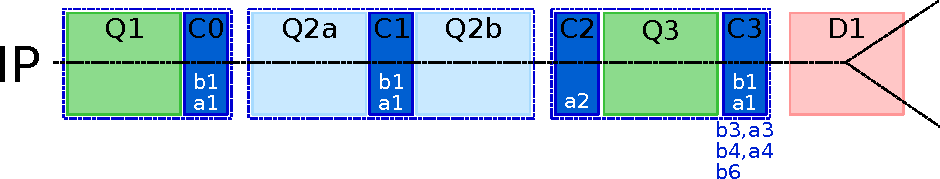
\includegraphics[height=2.5cm]{ir_lhc.pdf}
    \caption{Schematic of the right hand side of a LHC IR region and HL-LHC IR2 and IR8.
    Q1, Q2a/b and Q3 are the triplet quadrupoles.
    C0-C3 show the corrector packages with the field order to be corrected indicated. 
    The blue lines mark common cryostats. 
    The non-linear corrector package is included with the orbit correctors in C3.
    }
    \label{fig:irregionlhc}
\end{figure}


\begin{figure}[h!]
    \centering
    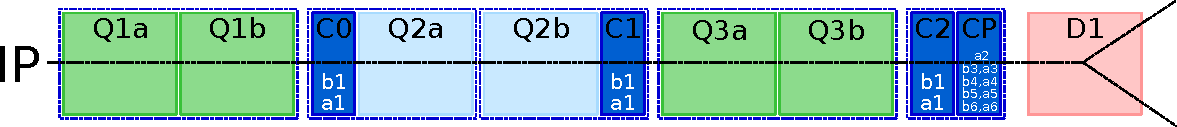
\includegraphics[width=\textwidth]{ir_hllhc.pdf}
    \caption{Schematic of the right hand side of HL-LHC IR1 and IR5.
    Q1a/b, Q2a/b and Q3a/b are the triplet quadrupoles. 
    C0, C1, C2 and CP show the corrector packages with the field order to be corrected indicated. 
    The blue lines mark common cryostats. 
    }
    \label{fig:irregionhllhc}
\end{figure}


\subsection{Resonance Driving Terms}

The transformation of the phase-space coordinates of a particle propagating through a circular accelerator 
can be described by means of maps, each describing the transformation generated by an element of the machine.
These maps are symplectic, i.e. they preserve phase-space volume, and can be combined, describing the propagation 
through multiple parts of the accelerator~\cite{DragtLieSeriesInvariant1976}, for example one complete turn. 

Using Lie-Algebra notation~\cite{DragtLieSeriesInvariant1976, DragtLieAlgebraicTheory1982}
%
\begin{equation}
    \label{eq:LieOperator}
    :f: = \sum\limits_{z=x,y} \frac{\partial f}{\partial z} \frac{\partial }{\partial p_z} - \frac{\partial f}{\partial p_z} \frac{\partial }{\partial z}
\end{equation}
%
a linear one turn map $\mathcal{M}$ can be transformed into a rotation $R$, its normal form:
\begin{equation}
    \label{eq:NormalizedTransformation}
    \mathcal{M} = e^{:h:}R  \; .
\end{equation}
%
In case of nonlinear elements present in the machine, the transformation becomes~\cite{ForestHamiltonianFreeDescription1990}:
\begin{equation}
    \label{eq:NormalFormTransformation}
    \mathcal{M} = e^{-:F:} \;  e^{:h:}R \; e^{:F:} \; .
\end{equation}

This transformation depends on the location $s$ at which the one-turn-map is calculated.
Truncating the exponential series at first order, it can be shown~\cite{TomasDirectMeasurementResonance2003} that
%
\begin{equation}
    \label{eq:hamiltonianTwissCoordinates}
    h(s) = \sum\limits_{jklm} h_{jklm}(s) \; (2J_x)^{\frac{j+k}{2}}(2J_y)^{\frac{l+m}{2}} e^{-i\left[(j-k)(\phi_x(s) + \phi_{x,0}) + (l-m)(\phi_y(s) + \phi_{y,0})\right]} \; ,
\end{equation}
%
with $\phi_{z}(s)$ being the phase in plane $z=x,y$ at $s$ and $\phi_{z, 0}$ the initial phase of the particle at injection.
$J$ is the action, i.e. the invariant of (linear) motion~\cite{CourantTheoryAlternatinggradientSynchrotron1958} and $h_{jklm}$ are the 
Hamiltonian coefficients~\cite{TomasDirectMeasurementResonance2003}, which 
are defined by all sources around the ring of multipole order $n = j + k + l + m$ (see \cref{sec:CorrectionPrinciple}).

The contribution $h_{jklm}$ from multipole sources of order $n \geq 2$ to the hamiltionian is given in 
\cite{FranchiStudiesMeasurementsLinear2006} Eq.~(3.11) as 
%
\begin{equation}
    \label{eq:HamiltonianTermsMultipoleSources}
    h_{jklm}(s) = 
    -\ReOf{    
     \frac{i^{l+m}}{j! \, k! \, l! \, m! \, 2^{j+k+l+m}}
    \beta_x(s)^{\frac{j+k}{2}}\beta_y(s)^{\frac{l+m}{2}} 
    \left(K_{n}(s) + iJ_{n}(s)\right)
     } \; .
\end{equation}
%
$K_n(s)$ and $J_n(s)$ are the magnetic field strengths of order $n$ at location $s$ of normal and skew fields respectively.
In this note, we use the convention of \textbf{starting the index $n$ at $1$, representing dipole fields} 
($n=2$ for quadrupole fields, etc.)

Similarly to $h(s)$, $F(s)$ is calculated as 
%
\begin{equation}
    \label{eq:NormalFormGeneratingFunction}
    F(s) = \sum\limits_{jklm} f_{jklm}(s) (2I_x)^{\frac{j+k}{2}}(2I_y)^{\frac{l+m}{2}} e^{-i\left[(j-k)(\psi_x(s) + \psi_{x,0}) + (l-m)(\psi_y(s) + \psi_{y,0})\right]} \; ,
\end{equation}
% 
with $I_z$ and $\psi_z$ being the action and angle coordinates of the nonlinear motion (called canonical coordinates of the normal form).
The generating terms $f_{jklm}$ of $F$ are the so called Resonance Driving Terms (RDTs) and it is shown 
in~\cite{ForestHamiltonianFreeDescription1990} (also given in \cite{FranchiStudiesMeasurementsLinear2006} Eq. (3.15)) that their relation to the hamiltonian terms is
%
\begin{equation}
    \label{eq:RDTHamiltonianRelation}
    f_{jklm}(s) = 
    \oint\limits_{\text{Ring}} \frac{h_{jklm}(s') \; (2J_x)^{\frac{j+k}{2}}(2J_y)^{\frac{l+m}{2}} 
    e^{-i\left[(j-k)\cdot\Delta\phi_x(s, s') + (l-m)\cdot\Delta\phi_y(s, s')\right]}}{1 - e^{-i2\pi[(j-k)Q_x + (l-m)Q_y]}} \;  \rm{d}s' \;.
\end{equation}
%
$\Delta\phi_z(s, s')$ is the phase advance in plane $z = x, y$ between $s$ and $s'$,
 while $Q_z$ are the horizontal and vertical tunes, i.e. the number of betatron oscillations per turn.


In case of the condition 
%
\begin{equation}
    \label{eq:ResonanceCondition}
    (j-k) \cdot Q_x + (l-m) \cdot Q_y = 2\pi \cdot p 
\end{equation}
%
being fulfilled for $p \in \mathbb{Z}$, $f_{jklm}$ diverges, if there are sources present for that order.
In this case the system is in a resonant state, and hence instable.
The behaviour of the instability as the systems approaches the resonance condition therefore depends 
on the strength of the multipole sources present in the machine.
Resonances labeled ($n_x$, $n_y$) are driven by all terms $n_x = j-k$ and $n_y = l - m$.

For each resonance ($n_x$, $n_y$) there is a line in the spectrum obtained by turn-by-turn beam position measurements,
which can be found at $-(n_x-1) \cdot Q_x - n_y \cdot Q_y$ (label: $(-n_x+1, -n_y)$)   in the spectrum of the horizontal plane 
and $-n_x \cdot Q_x - (n_y - 1) \cdot Q_y$ (label: $(-n_x, -n_y+1)$) in the spectrum of the vertical plane~\cite{FranchiStudiesMeasurementsLinear2006}.
The amplitude of these lines is proportional to $\left| f_{jklm} (s) \right|$~\cite{FranchiStudiesMeasurementsLinear2006},
the terms are therefore easily accessible from measurements~\cite{SchmidtMeasurementDrivingTerms2001,TomasDirectMeasurementResonance2003,TomasMeasurementGlobalLocal2005,FranchiFirstSimultaneousMeasurement2014,CarlierObservationsResonanceDriving2016}.

The $h_{jklm}$, and therefore $f_{jklm}$, are constant along $s$ until a multipole source of corresponding order is encountered,
at whose location its value jumps, which makes them very well suited as local observables~\cite{TomasMeasurementGlobalLocal2005}.
The correction algorithm presented here is based on locally minimizing the RDTs in the IR as shown in the next section. 

\subsection{Correction Principle}
\label{sec:CorrectionPrinciple}
 
In this section the correction principle as implemented in
the flexible correction algorithm v1.0.0 in~\cite{OMC-TeamIRNLRDTCorrection} is described.
The algorithm follows the simplifications of \cref{eq:HamiltonianTermsMultipoleSources,eq:RDTHamiltonianRelation} 
as outlined in~\cite{BruningDynamicApertureStudies2004}:

\begin{mytemize}
    \item Only the contribution from elements in one IR to the RDTs are minimized.
          The integral in \cref{eq:RDTHamiltonianRelation} includes therefore only IR elements.
    \item Constant coefficients of \cref{eq:RDTHamiltonianRelation} are ignored, 
          i.e. the numerator and actions as well as the coefficients depending only on $j,k,l,m$ and any signs,
          as they are not needed for minimization, .
    \item The phase of one side of the IR is approximately constant, as \\
          $\Delta \Phi(a,b) = \int\limits_a^b \frac{1}{\beta(s)} \rm{d}s$  
          and $\beta(s)$ being very large in the triplets. 
    \item The phase-advance between the left and right side of the IP is $\pi$. 
    \item The RDT is evaluated locally at the entrance of the IR. 
\end{mytemize}

With these approximations \cref{eq:RDTHamiltonianRelation} becomes an \textit{effective} RDT to minimize:
%
\begin{equation}
    \label{eq:effectiveRDT}
    f^\text{IR}_{jklm} =  \int\limits_\text{IR} 
    \ReOf{    
     i^{l+m}
     \left(K_{n}(s) + iJ_{n}(s) \right) 
    }
        \beta_x(s)^{\frac{j+k}{2}}
        \beta_y(s)^{\frac{l+m}{2}} 
     e^{i \pi n \theta(s - s_\text{IP})}
    \rm{d}s \; ,
\end{equation}
%
with $\theta(x)$ being the heaviside step function and $s_\text{IP}$ the location of 
the IP within the IR.
The $n$ in the exponent replaces $j - k + l - m = n - 2k - 2l$, 
as for even (odd) n, this value will also be even (odd), 
independent of the particular choices for $j,k,l,m$.

The main concept of the correction is then to find the $K_n(s)$ and $J_n(s)$ of 
the corrector magnets, that minimize a set of given $f^\text{IR}_{jklm}$ based on given optics.

As there are usually two correctors per multipole field available (one on each side of the IP), 
two combinations of $l+m$ and $j+k$ (the exponents of the $\beta$ function)
can be corrected.
As the correctors are responsible for the correction of both beams, 
the exponents need to be chosen such that the correction is valid for both beams, 
which means that only a single RDT per beam can be corrected 
unless the symmetry of the optics can be used to correct
two RDTs (see \cref{sec:DualOptics}).

In the LHC $a_3, b_3, a_4, b_4$ and $b_6$ correctors are available,
in the HL-LHC additionally $a_5, b_5$ and $a_6$.


\subsubsection{Equation System}

In our simulations, the input to the correction algorithm will be the output 
of \ttt{TWISS} and \ttt{ESAVE} functions from \ttt{MAD-X}~\cite{CERNMadX}.
These are tables in which $K_n(s)$ and $J_n(s)$ are not continuous functions, 
but given as already integrated values $K_nL_w$, $J_nL_w$ 
(\ttt{K$_{n-1}$L}, \ttt{K$_{n-1}$SL} in the terminology of \ttt{MAD-X}) for each element $w$.
Values for the longitudinal position $s_w$, $\beta_{x,w}, \beta_{x,w}$ and the transversal orbit $x_w, y_w$, which will be important 
when calculating feed-down (see below), are also provided.


To assure aa accurate estimate for the integral in \cref{eq:effectiveRDT}, 
the lattice should be \textit{sliced} in \ttt{MAD-X}, 
i.e. all magnets are approximated by single kicks surrounded by drift-spaces. 
Long magnets should be cut into multiple of these slices to increase accuracy. 
Corrector magnets on the other hand, which are in any case short compared to e.g. dipoles, 
can  be represented by a single slice.

In this thin-lens approximation, \cref{eq:effectiveRDT} transforms into a sum over all elements (slices) $w$ in the IR, 
which needs to be set to zero to suppress the RDT:
 %
\begin{equation}
    \label{eq:effectiveRDTSum}
    f^\text{IR}_{jklm} =  \sum\limits_{w \in \text{IR}} 
    \ReOf{    
     i^{l+m}
     \left(K_{n}L_w + iJ_{n}L_w \right) 
    }
        \beta_{x,w}^{\frac{j+k}{2}}
        \beta_{y,w}^{\frac{l+m}{2}} 
     e^{i \pi n \theta(s_w - s_\text{IP})} 
     \overeq{!} 0 
     \; .
\end{equation}
%

Splitting the elements into corrector elements $\mathcal{C}$ and non-corrector elements $\text{IR}\setminus\mathcal{C}$,
\cref{eq:effectiveRDTSum} transforms into:
 %
\begin{equation}
    \label{eq:equationSum}
    \begin{split}
    &\sum\limits_{w \in \mathcal{C}} 
    \ReOf{    
     i^{l+m}
     \left(K_{n}L_w + iJ_{n}L_w \right) 
    }
        \beta_{x,w}^{\frac{j+k}{2}}
        \beta_{y,w}^{\frac{l+m}{2}} 
     e^{i \pi n \theta(s_w - s_\text{IP})} \\
     = 
    -&\sum\limits_{w \in \text{IR}\setminus\mathcal{C}} 
    \ReOf{  
     i^{l+m}
     \left(K_{n}L_w + iJ_{n}L_w \right) 
    }
        \beta_{x,w}^{\frac{j+k}{2}}
        \beta_{y,w}^{\frac{l+m}{2}} 
     e^{i \pi n \theta(s_w - s_\text{IP})} 
    \end{split}
     \; ,
\end{equation}

It is important to note, that each corrector is defined by either
$K_nL$ or $J_nL$, so that per order $n$ and orientation (normal, skew) only a limited set of 
correctors is left.
Normally there are two of these correctors in the LHC/HL-LHC, i.e. one per IP side,
and $\mathcal{C} = \{cl, cr\}$, a left ($cl$) and a right ($cr$) corrector element.
Defining the sum over IR$\setminus\mathcal{C}$ in \cref{eq:equationSum}
as $I_{jklm}$ and
\begin{equation}
    \label{eq:BcomponentsDef}
    \begin{split}
    b_{jklm}^{(cl)} &= 
     \hphantom{(-1)^n} \, i^{l+m} \,
     \beta_{x,cl} ^{\frac{j+k}{2}} \beta_{y,cl}^{\frac{l+m}{2}} 
    \\
    b_{jklm}^{(cr)} &= 
     (-1)^n\, i^{l+m} \, 
     \beta_{x,cr} ^{\frac{j+k}{2}} \beta_{y,cl}^{\frac{l+m}{2}} \; ,
    \end{split}
\end{equation}
%
\cref{eq:equationSum} can be split into a two equation system 
%
\begin{equation}
    \label{eq:linearEqSystemSingle}
    \begin{split}
        \begin{pmatrix}
            b_{jklm}^{(cl)} & b_{jklm}^{(cr)}
        \end{pmatrix}
        \begin{pmatrix}
            K_{n}L_{cl} \\ 
            K_{n}L_{cr}
        \end{pmatrix}
        &= - I_{jklm}
        \qquad \text{if } l+m \text{ even},
        \\
        \begin{pmatrix}
            i \, b_{jklm}^{(cl)} & i \, b_{jklm}^{(cr)}
        \end{pmatrix}
        \begin{pmatrix}
            J_{n}L_{cl} \\ 
            J_{n}L_{cr}
        \end{pmatrix}
        &= - I_{jklm}
        \qquad  \text{if } l+m \text{ odd}, 
    \end{split}
\end{equation}
%
which can be easily extended to include multiple RDTs, e.g.:
\begin{equation}    
    \label{eq:linearEqSystemDouble}
        \begin{pmatrix}
            b_{jklm}^{(cl)} & b_{jklm}^{(cr)} \\
            b_{j'k'l'm'}^{(cl)} & b_{j'k'l'm'}^{(cr)}
        \end{pmatrix}
        \begin{pmatrix}
            K_{n}L_{cl} \\ 
            K_{n}L_{cr}
        \end{pmatrix}
        = - 
        \begin{pmatrix}
            I_{jklm} \\ 
            I_{j'k'l'm'} 
        \end{pmatrix}
\end{equation}
with $j+k+l+m = j'+k'+l'+m' = n$ and $l + m$ and $l'+m'$ both even.
These linear equation systems can be solved or optimized for $K_nL_{cl, cr}$ or $J_nL_{cl, cr}$ by standard algorithms.


\subsubsection{Dual Optics} % --------------------
\label{sec:DualOptics}

% \begin{tikzpicture}
%     \node (start) at (0, 0) {aaa};
%     \node (end) at (1, 1) {bbb};
%     \draw[red, ->]  (start) -- (end);
% \end{tikzpicture}


\begin{figure}[htbp]
    \centering
    \begin{subfigure}{0.35\textwidth}
        % 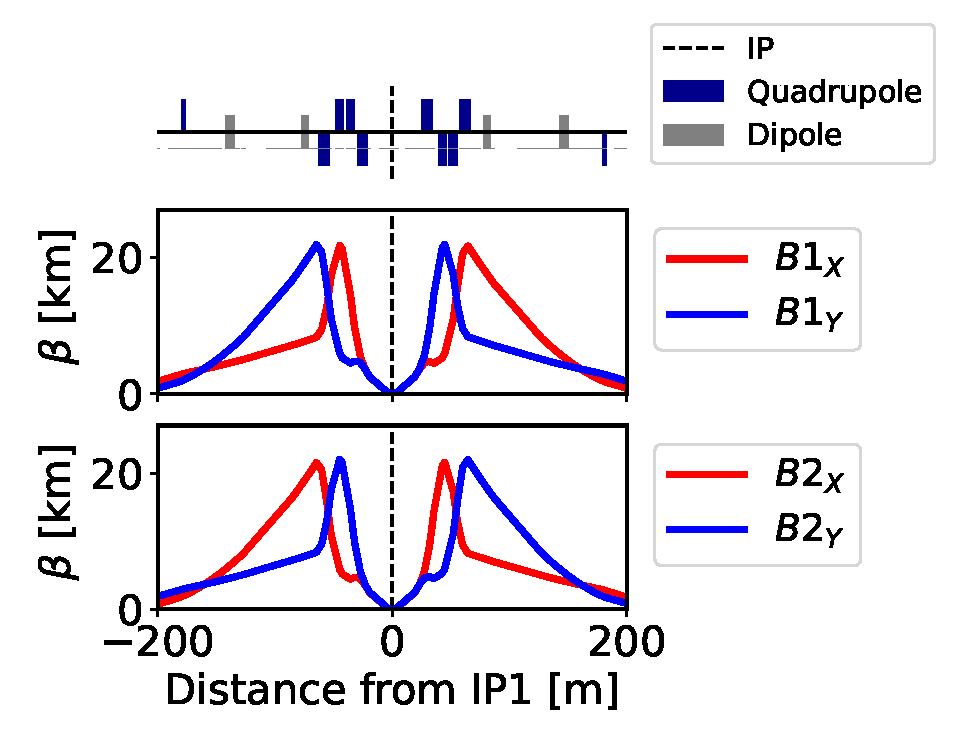
\includegraphics[height=60mm,trim=15 0 160 0, clip]{images/optics/plot.hllhc.round1515.xing_top.beta.IP1.pdf}
        \begin{tikzpicture}[every node/.style={inner sep=1pt,outer sep=0}]
            \node (image) at (current page.center) {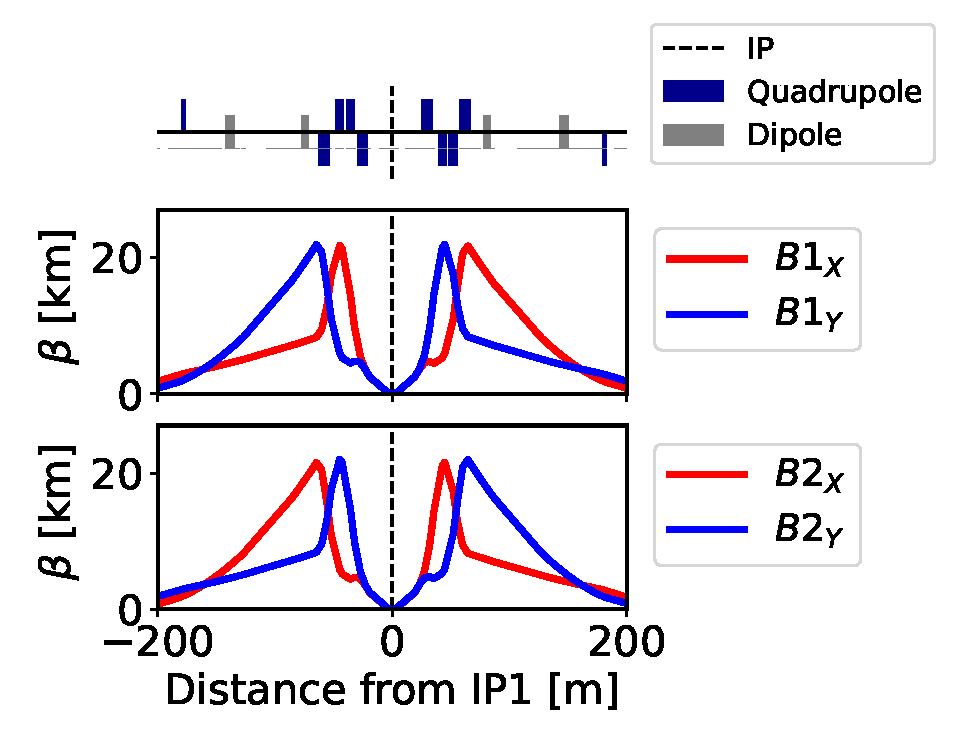
\includegraphics[height=60mm, trim=15 0 160 0, clip]{images/optics/plot.hllhc.round1515.xing_top.beta.IP1.pdf}};
            \begin{scope}[shift={(image.south west)},x={(image.south east)},y={(image.north west)}]
            \node (b1start) at (0.238, 0.454){};
            \node (b1)[right= 10pt of b1start] {\tiny Beam 1};
            \node (b1end)[right= 10pt of b1]{};
            \draw[-]  (b1start) -- (b1);
            \draw[->]  (b1) -- (b1end);
            \node (b2start) at (0.94, 0.454){};
            \node (b2)[left= 10pt of b2start] {\tiny Beam 2};
            \node (b2end)[left= 10pt of b2]{};
            \draw[-]  (b2start) -- (b2);
            \draw[->]  (b2) -- (b2end);
            \end{scope}
        \end{tikzpicture}
        \caption{$\beta^* = \qty{15}{cm}$ round optics}
        \label{fig:betaIP1HLLHCround}
    \end{subfigure}
    \begin{subfigure}{0.35\textwidth}
        % 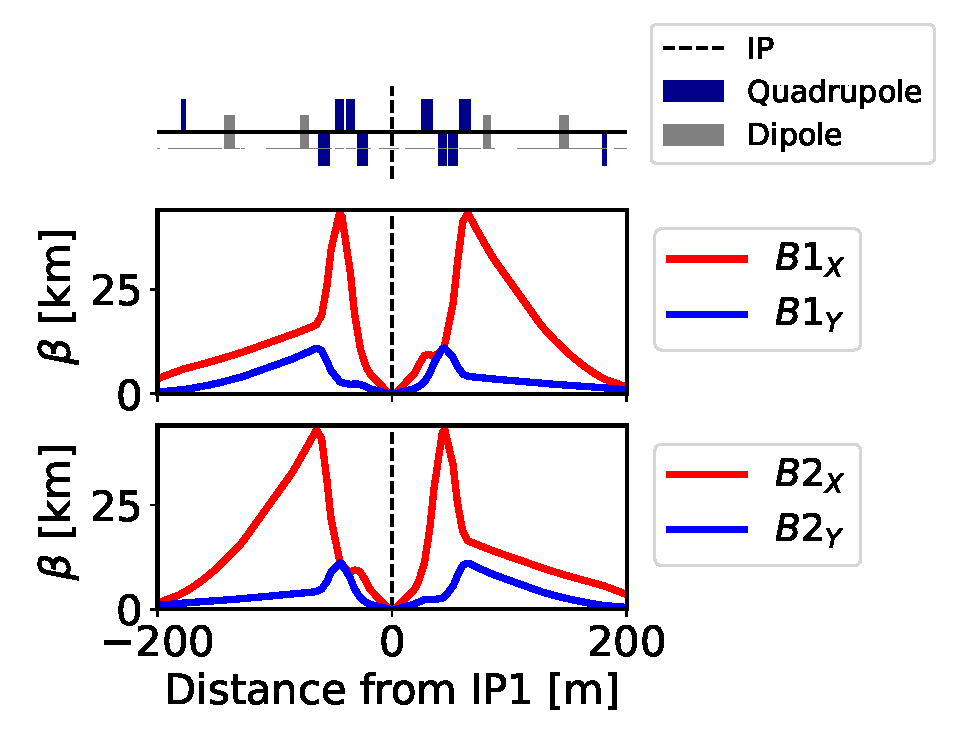
\includegraphics[height=60mm, trim=40 0 19 0, clip]{images/optics/plot.hllhc.flat07530.xing_top.beta.IP1.pdf}
        \begin{tikzpicture}[every node/.style={inner sep=1pt,outer sep=0}]
            \node (image) at (current page.center) {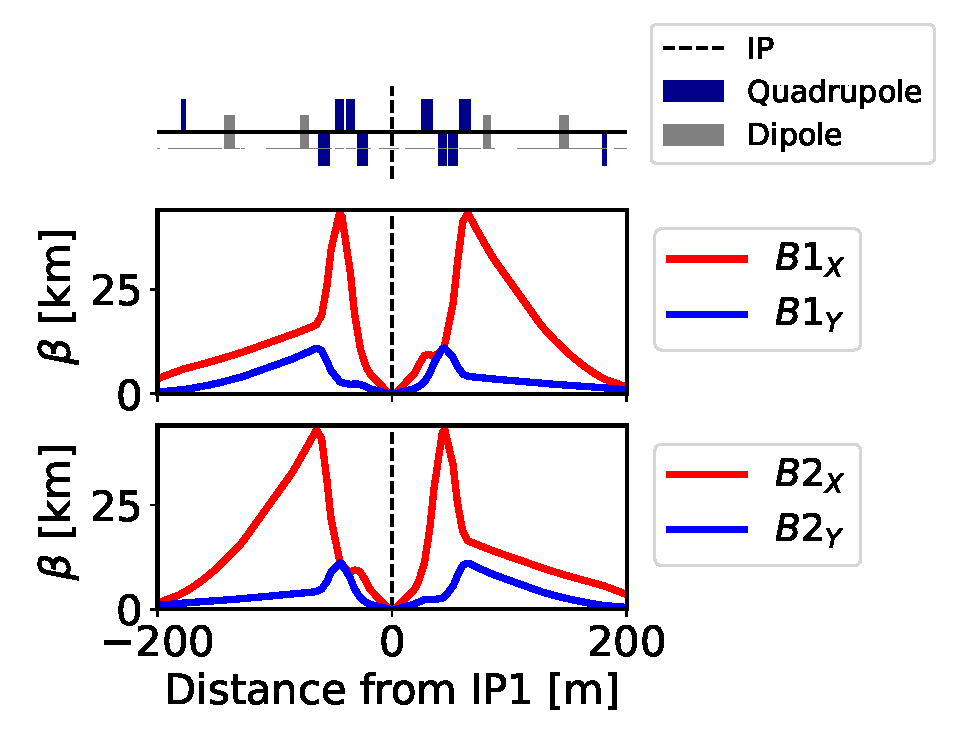
\includegraphics[height=60mm, trim=40 0 19 0, clip]{images/optics/plot.hllhc.flat07530.xing_top.beta.IP1.pdf}};
            \begin{scope}[shift={(image.south west)},x={(image.south east)},y={(image.north west)}]
            \node (b1start) at (0.107, 0.454){};
            \node (b1)[right= 10pt of b1start] {\tiny Beam 1};
            \node (b1end)[right= 10pt of b1]{};
            \draw[-]  (b1start) -- (b1);
            \draw[->]  (b1) -- (b1end);
            \node (b2start) at (0.62, 0.454){};
            \node (b2)[left= 10pt of b2start] {\tiny Beam 2};
            \node (b2end)[left= 10pt of b2]{};
            \draw[-]  (b2start) -- (b2);
            \draw[->]  (b2) -- (b2end);
            \end{scope}
        \end{tikzpicture}
        \caption{$\beta^* = \qty{7.5}{cm}/\qty{30}{cm}$ flat optics}
        \label{fig:betaIP1HLLHCflat}
    \end{subfigure}
	\caption{HL-LHC $\beta$-functions in the IR around IP1.}
	\label{fig:betaIP1HLLHC}
\end{figure}

In the original implementation of the algorithm in~\cite{BruningDynamicApertureStudies2004},
the optics of only one beam could be given and the algorithm was making use 
of the symmetries of the $\beta$-function in the IR
%
\begin{equation}
    \label{eq:betaSymmetriesRound}
    \begin{split}
        \beta_x^{\text{(B1)}}(s) &= \beta_y^{\text{(B2)}}(s) \\ 
        \beta_y^{\text{(B1)}}(s) &= \beta_x^{\text{(B2)}}(s) \;, 
    \end{split}
\end{equation}
%
which is true for round optics as shown in~\cref{fig:betaIP1HLLHCround}, to calculate a correction valid for both beams.
With this symmetry the effective RDT \cref{eq:effectiveRDT} simply switches the $\beta$ exponents between the beams, 
for which we will use the notation
%
\begin{equation}
    \label{eq:effectiveRDT*}
    f^\text{IR (B1)}_{jklm*}  
    \quad \overeq{\cref{eq:effectiveRDT}} \quad
    \int\limits_\text{IR} 
    \ReOf{ 
     i^{l+m}
     \left(K_{n}(s) + iJ_{n}(s) \right) 
    }
        \beta_x(s)^{\frac{l+m}{2}}
        \beta_y(s)^{\frac{j+k}{2}} 
     e^{i \pi n \theta(s - s_\text{IP})}
    \rm{d}s 
    \quad \overeq{\cref{eq:betaSymmetriesRound}} \quad
    f^\text{IR (B2)}_{lmjk}\; .
\end{equation}
%
As mentioned in the previous section, with the two correctors per field type (order and orientation),
we can perfectly correct two RDTs locally in the IR. 
When 
%
\begin{equation}
    j+k \equiv l+m \mod{2} \;,
\end{equation}
%
i.e. both $f_{jklm}$ and $f_{lmjk}$ are skew (normal) RDTs, 
two RDTs per beam can be corrected: 
$f^\text{IR}_{jklm*} = \pm f^\text{IR}_{lmjk}$ within the optics of the same beam
and we can therefore choose $f^\text{IR}_{j'k'l'm'}  = f^\text{IR}_{lmjk} (= \pm f^\text{IR}_{jklm*})$ in \cref{eq:linearEqSystemDouble}.
If on the other hand $j+k$ and $l+m$ are of different parity, only \textbf{one} RDT $f^\text{IR}_{jklm}$ per beam can be corrected, 
by targeting $f^\text{IR}_{jklm}$ and $f^\text{IR}_{j'k'l'm'} = f^\text{IR}_{jklm*}$ in the given optics.

There are optics in which \cref{eq:betaSymmetriesRound} does not hold true anymore.
For example, in contrast to \textit{round} optics, 
in which the $\beta$-function  at the IP ($\beta^* = \beta(s_\text{IP})$) is equal for both transversal planes ($\beta^*_x = \beta^*_y$),
there exists also so called \textit{flat} optics, for which $\beta^*_x \neq \beta^*_y$ 
(i.e. the beam shape is \textit{flat} at the IP)~\cite{FartoukhAchromaticTelescopicSqueezing2013,FartoukhFlatTelescopicOptics2018}.
A realization of flat optics, forseen to be used in the HL-LHC, is shown in \cref{fig:betaIP1HLLHCflat}.

The straightforward way to not to rely on \cref{eq:betaSymmetriesRound}, 
is to use the optics for both beams in the correction and construct \cref{eq:linearEqSystemDouble} from both
%
\begin{equation}    
    \label{eq:linearEqSystemDoubleOptics}
        \begin{pmatrix}
            b_{jklm}^{(cl, \text{B1})} & b_{jklm}^{(cr, \text{B1})} \\
            b_{jklm}^{(cl, \text{B2})} & b_{jklm}^{(cr, \text{B2})}
        \end{pmatrix}
        \begin{pmatrix}
            K_{n}L_{cl} \\ 
            K_{n}L_{cr}
        \end{pmatrix}
        = - 
        \begin{pmatrix}
            I^{(\text{B1})}_{jklm} \\ 
            I^{(\text{B2})}_{jklm} 
        \end{pmatrix} 
        \; .
\end{equation}

\subsubsection{Feed-Down} % --------------------

The effect of feed-down occurs whenever a particle beam is passing off-center through a magnet, 
due to either a transverse misalignment of the magnet or an off-center closed orbit of the beam itself.
In these cases, the magnetic field can be described via Taylor expansion as a composition of 
magnetic field components with identical geometry as lower order fields in addition to the current field of higher order. 
These components therefore cause the same effects on the beam 
as lower order sources would~\cite{WiedemannParticleAcceleratorPhysics2015}. 

Feed-down can be understood by applying a first-order Taylor Expansion $x \mapsto x + \Delta x$ and $y \mapsto y + \Delta y$
to \cref{eq:hamiltonianTwissCoordinates} in the 
curvilinear (comoving) coordinate system
%
\begin{equation}
   \label{eq:hamiltonianFeeddownDerivation}
   \begin{split}
   h
   &= \qquad 
   -\ReOf{\sum_{n = 2}^\infty \left(K_n + iJ_n\right)\frac{\left(x+iy\right)^n}{n!}} \\
   &\overeq{Taylor} \qquad
    -\ReOf{
        \sum_{n = 2}^\infty (K_n + iJ_n)
        \frac{\sum\limits_{q=0}^{n} \frac{1}{q!} \frac{n!}{(n-q)!}(x+iy)^{n-q} (\Delta x + i \Delta y)^q}{n!}
    } \\
    &=\qquad
     -\ReOf{
         \sum_{n = 2}^\infty (K_n + iJ_n)
         \sum\limits_{q = 0}^{n} \frac{(x+iy)^{n-q} (\Delta x + i \Delta y)^q}{q!\, (n-q!)} 
      } \\
     &\myoverunder{\text{sort by } (x + iy)^n}{=}{n \mapsto n+q} \qquad
     - \ReOf{
        \sum_{n = 0}^\infty \sum_{\substack{q=0 \text{ if } n \geq 2 \\ q = 2 \text{  if } n < 2 }}^{\infty} \frac{1}{q!\, n!}
        (K_{n+q} + iJ_{n+q}) (x + iy)^n (\Delta x + i \Delta y)^q 
     } \\
     &= \qquad
     - \ReOf{\sum_{n = 0}^\infty 
        \left( \sum_{\substack{q=0 \text{ if } n \geq 2 \\ q = 2 \text{  if } n < 2 }}^{\infty} 
        (K_{n+q} + iJ_{n+q}) \frac{(\Delta x + i \Delta y)^q}{q!} \right)
        \frac{(x + iy)^n}{n!}
     }
   \end{split}
\end{equation}
%
For brevity $(s)$ is omitted, but $h, K_n, J_n, x, y$ and $\Delta x, \Delta y$ are all dependent on the longitudinal location.
From \cref{eq:hamiltonianFeeddownDerivation} one can see that magnetic field strengths
of order $n \geq 2$ without feed-down are replaced by a sum depending  on the deviation of the beam from 
magnet-center and higher order field strengths.
Feed-down to field order $n \geq 2$ from fields up to $n + Q$ can now be calculated by:
%
\begin{equation}
    \label{eq:feeddownOrderN}
    K_n + iJ_n \overset{\text{w/ feeddown}}{\rightarrow} \sum_{q = 0}^{Q} (K_{n+q} + iJ_{n+q}) \frac{(\Delta x + i \Delta y)^q}{q!}.
\end{equation}
%
Fields feed-down can also have an effect on the scalar field ($n = 0$) and dipole fields ($n = 1$).
As their structure does not follow the structure in \cref{eq:hamiltonianTwissCoordinates},
\cref{eq:feeddownOrderN} is not applicable.
In the context of RDTs $n$ is always larger than 2 and we can use \cref{eq:feeddownOrderN} 
in the definition of the effective RDT \cref{eq:effectiveRDT}
%
\begin{equation}
    \label{eq:effectiveRDTfeeddown}
    \small
    f^\text{IR}_{jklm} =  \int\limits_\text{IR} 
    \ReOf{    
     i^{l+m}
     \sum_{q = 0}^{\infty} 
     (K_{n+q}(s) + iJ_{n+q}(s)) \frac{(\Delta x(s) + i \Delta y(s))^q}{q!} 
    }
        \beta_x(s)^{\frac{j+k}{2}}
        \beta_y(s)^{\frac{l+m}{2}} 
     e^{i \pi n \theta(s - s_\text{IP})}
    \rm{d}s \; ,
\end{equation}
%
and can therefore easily include it when building the equation systems 
\cref{eq:linearEqSystemSingle}, \cref{eq:linearEqSystemDouble} or \cref{eq:linearEqSystemDoubleOptics}.

Not only can feed-down be used to calculate the influence of field errors of orders $\geq n$ on the RDT, 
i.e. by contributing to the integral $I_{jklm}$, but it can also be used to calculate the strengths 
of correctors of orders $n_\text{Corrector} > n$ to counteract the RDT via feed-down.
The matrix elements of the corrector coefficients in \cref{eq:BcomponentsDef} will then also contain the feed-down coefficient
%
\begin{equation}
    \label{eq:zpDefinition}
    z_{p} = \frac{\left( \Delta x + i\Delta y\right)^p}{p!} \, \,
\end{equation}
%
with $p$ being the order of feed-down necessary, i.e. 
\begin{equation}
    \label{eq:DiffOrderCorrectorRDT}
    p = n_\text{Corrector} - n \, .
\end{equation}
%
As $z_p \in \mathbb{C}$, this makes the evaluation of the real part in \cref{eq:equationSum}, 
needed to split the equation system into two, separating the correctors (\cref{eq:linearEqSystemSingle}), 
less straightforward and more cases need to be considered.
Inserting
%
\begin{equation}
    \label{eq:KnJnWithZp}
    \begin{split}
        &\ReOf{    
        i^{l+m}
        (K_{n+p}L_w + iJ_{n+p}L_w) \frac{(\Delta xL_w + i \Delta yL_w)^q}{q!} 
        }
        \\
        \overeq{\cref{eq:zpDefinition}} \quad
        &\ReOf{    
        i^{l+m}
        (K_{n+p}L_w + iJ_{n+p}L_w) \cdot z_p 
        }
        \\
        =  \quad
        &\ReOf{    
        i^{l+m}
        (K_{n+p}L_w + iJ_{n+p}L_w) (\ReOf{z_p} + i\ImOf{z_p}) 
        }
        \\
        =  \quad
        &\ReOf{    
        i^{l+m} \left[
        (K_{n+p}L_w \cdot \ReOf{z_p} -J_{n+p}L_w \cdot \ImOf{z_p}) + i(K_{n+p}L_w \cdot \ImOf{z_p} + J_{n+p} \cdot \ReOf{z_p} )\right] 
        }
    \end{split}
\end{equation}
%
into \cref{eq:equationSum} yields the equation system
%
\begin{equation}
    \label{eq:linearEqSystemFeeddown}
    \begin{split}
    \footnotesize
    \begin{pmatrix}
        \ReOf{z_p} \cdot b_{jklm}^{(cl)} & 
        \ReOf{z_p} \cdot b_{jklm}^{(cr)} & 
        -\ImOf{z_p} \cdot b_{jklm}^{(cl)} &
        -\ImOf{z_p} \cdot b_{jklm}^{(cr)}
    \end{pmatrix}
    \begin{pmatrix}
        K_{n+p}L_{cl} \\ 
        K_{n+p}L_{cr} \\ 
        J_{n+p}L_{cl} \\ 
        J_{n+p}L_{cr}
    \end{pmatrix}
     &= -
     I_{jklm} \quad
    \text{for even } l+m, 
     \\
    \footnotesize
    \begin{pmatrix}
        i \,\ImOf{z_p} \cdot b_{jklm}^{(cl)} & 
        i \,\ImOf{z_p} \cdot b_{jklm}^{(cr)} & 
        i \,\ReOf{z_p} \cdot b_{jklm}^{(cl)} & 
        i \,\ReOf{z_p} \cdot b_{jklm}^{(cr)}
    \end{pmatrix}
    \begin{pmatrix}
        K_{n+p}L_{cl} \\ 
        K_{n+p}L_{cr} \\ 
        J_{n+p}L_{cl} \\
        J_{n+p}L_{cr}
    \end{pmatrix}
     &=  
     -I_{jklm} \quad
    \text{for odd } l+m \; .
    \end{split}
\end{equation}
%
In the case of $p = 0$, \cref{eq:linearEqSystemFeeddown} transforms back to \cref{eq:linearEqSystemSingle},
as $\ReOf{z_0} = 1$ and $\ImOf{z_0} = 0$. 
For simplicity, we can redefine $b_{jklm}$ to include the additional factors directly into the coefficients 
\begin{equation}
    \label{eq:coefficientWithFeeddown}
    b_{jklm,p} =
    \begin{cases}
      \phantom{-} \ReOf{z_p} \cdot b_{jklm}   \quad \text{if normal corrector and } l + m \text{ even}, \\
     \phantom{-} \ImOf{z_p} \cdot b_{jklm}    \quad \text{if normal corrector and } l + m \text{ odd}, \\    
      -\ImOf{z_p} \cdot b_{jklm}              \quad \text{if skew corrector and } l + m \text{ even}, \\    
       \phantom{-} \ReOf{z_p}  \cdot b_{jklm} \quad \text{if skew corrector and } l + m \text{ odd} 
    \end{cases}
\end{equation}
%
and take care to take $z_p$ into account, whenever $p>0$.

Including feed-down into the equation system also allows therefore to correct multiple orders of RDTs with the same correctors, 
as well as correcting RDTs with correctors of multiple orders.
\Cref{eq:linearEqSystemSingle} can hence not only be extended ``vertically'' by correcting for multiple beam optics (\cref{eq:linearEqSystemDoubleOptics})
 and different RDTs (\cref{eq:linearEqSystemDouble}) at the same time, 
but also ``horizontally'', by adding more correctors, e.g.
%
\begin{equation}    
    \label{eq:linearEqSystemDoubleCorrectors}
        \begin{pmatrix}
            b_{jklm}^{(cl)} & b_{jklm}^{(cr)} & b_{jklm,p}^{(cl)} & b_{jklm,p}^{(cr)} \\
            b_{j'k'l'm'}^{(cl)} & b_{j'k'l'm'}^{(cr)} & b_{j'k'l'm',p}^{(cl)} & b_{j'k'l'm',p}^{(cr)}
        \end{pmatrix}
        \begin{pmatrix}
            K_{n}L_{cl} \\ 
            K_{n}L_{cr} \\
            K_{n+p}L_{cl} \\ 
            K_{n+p}L_{cr}
        \end{pmatrix}
        = - 
        \begin{pmatrix}
            I_{jklm} \\ 
            I_{j'k'l'm'} 
        \end{pmatrix}
\end{equation}

% Implementation Details %%%%%%%%%%%%%%%%%%%%%%%%%%%%%%%%%%%%%%%%%%%%%%%%%%%%%%%%%%%%%%%%%%%%%%%%%%%%%% 
\FloatBarrier
\section{Implementation}
This chapter describes the implementation of the correction algorithm as 
realized in Version 1.0.0 of \cite{OMC-TeamIRNLRDTCorrection}.
Direct links to lines of the code as well as usage of \ttt{python} is avoided,
yet the structure and naming of the sections in this chapter is kept close to the names in the actual code,
which can be found on
\href{https://github.com/pylhc/irnl_rdt_correction}{https://github.com/pylhc/irnl\_rdt\_correction}.
The API is documented in  
\href{https://pylhc.github.io/irnl_rdt_correction}{https://pylhc.github.io/irnl\_rdt\_correction}.

\begin{important}
        \item[\color{CernRed} Attention] While this note follows the convention of \textbf{n = 1 for dipole fields}, 
        in the code the \ttt{MAD-X} convention of \textbf{n = 0 for dipole fields}  is used, as the input will already be in that format.
\end{important}

\myparagraph{Dependencies}

The package is mostly self-contained and depends only on:

\begin{options}
        \item[numpy]
        provides an easy way to work with numerical data in arrays as well as additional functionality 
        e.g. for solving linear equation systems~\cite{HarrisArrayProgrammingNumPy2020}.
        \item[pandas]
        allows working with data-tables, which are used to structure the data and allow easy access and identification 
        of the different optics parameters~\cite{pandas}.
        \item[tfs-pandas]
        a wrapper for \opt{pandas} to read tables from  and write tables into files of 
        the Table File System (TFS) format used by \ttt{MAD-X}~\cite{CERNMadX}~\cite{OMC-TeamTFSPandas}.
\end{options}


\subsection{Beam Directions}
\label{sec:BeamDirection}

\begin{figure}[h!]
    \centering
    \begin{subfigure}{0.4\textwidth}
        % 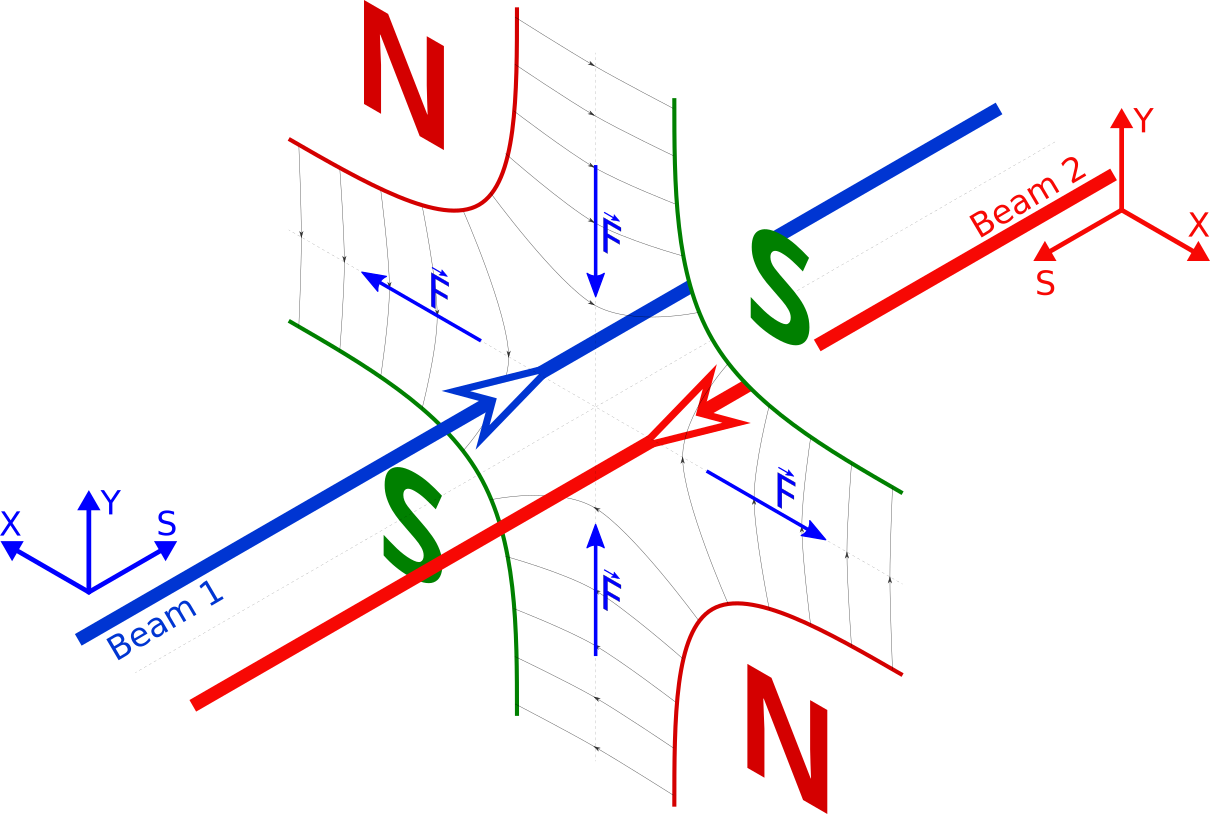
\includegraphics[width=\textwidth]{beamDirection/quadBeam1.png}
        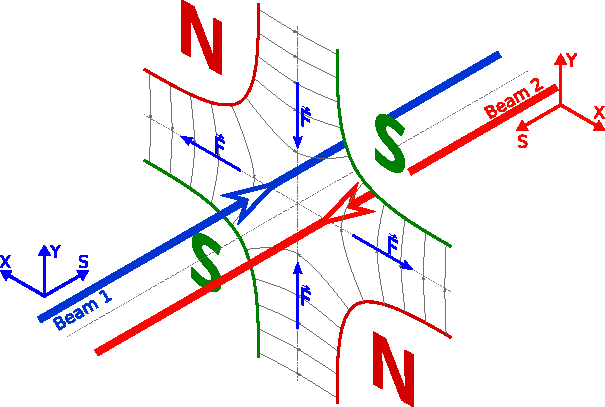
\includegraphics[width=\textwidth]{beamDirection/quadBeam1.pdf}
        \caption{In reference frame of Beam~1}
    \end{subfigure}
    \hspace{2em}
    \begin{subfigure}{0.4\textwidth}
        % 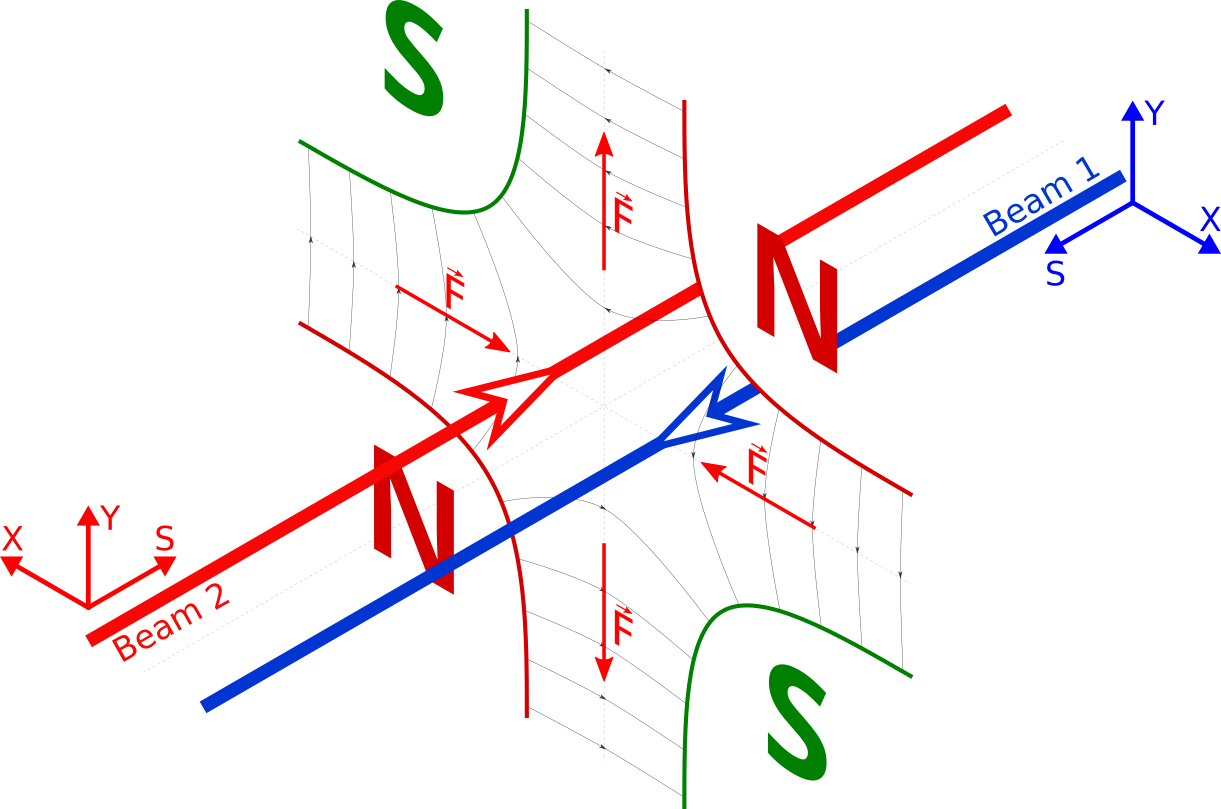
\includegraphics[width=\textwidth]{beamDirection/quadBeam2.png}
        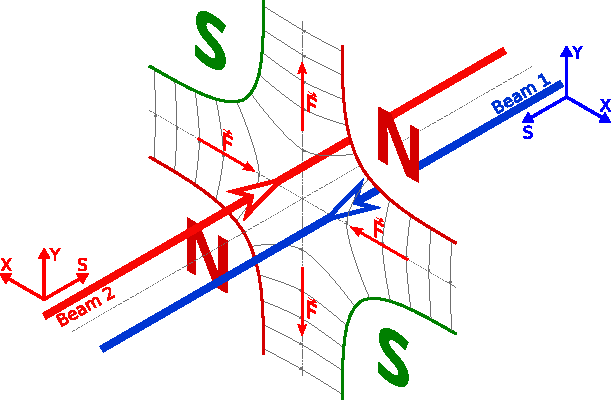
\includegraphics[width=\textwidth]{beamDirection/quadBeam2.pdf}
        \caption{In reference frame of Beam~2}
    \end{subfigure}
    \caption{Schematic of two beams traveling in opposite directions through a quadruople.}
    \label{fig:BeamDirection}
\end{figure}

Because of the opposite traveling direction of Beam~2, magnetic fields in the reference frame of this beam look as if rotated
by \qty{180}{\degree} around the y-axis at the center of the magnet, compared to the reference frame of Beam~1.
Hence magnets that are symmetric upon this rotation will have the same effect on the beams, 
while magnets that are not symmetric will look like they have opposite-sign field gradients,
e.g. a focusing quadrupole magnet with strength $K_2$ in Beam~1 is seen as a defocusing magnet with $-K_2$ in Beam~2 
(as they are anti-symmetric upon the \qty{180}{\degree} rotation around the y-axis with respect to their polarity, see \cref{fig:BeamDirection}).
%
In general:
%
\begin{equation}
\label{eq:B1toB2}
(K_n + iJ_n)^\text{B2} =
\begin{cases}
        (-K_n + iJ_n)^\text{B1} \; , \text{if } n \text{ is even} \\
        (\phantom{-}K_n - iJ_n)^\text{B1} \; , \text{if } n \text{ is odd} \;.
\end{cases}
\end{equation}
%
This becomes important as soon as both beams need to be corrected by the same (i.e. single aperture) correctors, 
especially as there are two different definitions for Beam~2 in \ttt{MAD-X}: 
One called is ``Beam~2'', 
for which all elements are defined in the reference frame of Beam~1 
and the beam direction is handled via a negative beam velocity (\ttt{BV=-1}); 
the other one is called ``Beam~4'' and here the whole lattice is inverted and the beam travels in forward direction (\ttt{BV=1}),
which means the field strengths follow the relation in \cref{eq:B1toB2}.
Quotes are kept in the following, to indicate that this is not Beam~2 as in the machine, 
but ``Beam~2'' or ``Beam~4''as defined in \ttt{MAD-X}.
The lattice for ``Beam~1'' in \ttt{MAD-X} follows the beam direction of Beam~1 in the actual machine.
One should note, that the beam direction is already taken into account in the field strength data of \ttt{TWISS} 
in \ttt{MAD-X}, but not in the \opt{errors} output of \ttt{ESAVE} and not in the horizontal orbit, the \ttt{X} and \ttt{DX} data respectively.
To assure consistent behaviour, the optics of ``Beam~2'' are brought into the reference frame of ``Beam~4'' upon loading.

When building an equation system as in \cref{eq:linearEqSystemDoubleOptics}, the reference frame needs again to be taken into account:
\Cref{eq:linearEqSystemDoubleOptics} is only correct, when all values are calculated in the same reference frame.  
As they are not, each line in \cref{eq:linearEqSystemDoubleOptics} is correct in its own reference frame, 
but the $K_nL$ and $J_nL$ values are shared between the two frames. 
To account for the appropriate signs, the signs of the coefficients are inverted according to \cref{eq:B1toB2} where needed for Beam~2: 
%
\begin{equation}    
    \label{eq:linearEqSystemDoubleOpticsBeamDirection}
    \begin{split}
        \begin{pmatrix}
            b_{jklm}^{(cl, \text{B1})} & b_{jklm}^{(cr, \text{B1})} \\
            \pm b_{jklm}^{(cl, \text{B2})} & \pm b_{jklm}^{(cr, \text{B2})}
        \end{pmatrix}
        \begin{pmatrix}
            K_{n}L_{cl} \\ 
            K_{n}L_{cr}
        \end{pmatrix}
        = -
        \begin{pmatrix}
            I^{(\text{B1})}_{jklm} \\ 
            I^{(\text{B2})}_{jklm} 
        \end{pmatrix} 
        \quad \text{if} \; n \; \text{is} \; \{\substack{\text{odd}\\\text{even}} \;,
        \\ 
        \begin{pmatrix}
            ib_{jklm}^{(cl, \text{B1})} & ib_{jklm}^{(cr, \text{B1})} \\
            \pm ib_{jklm}^{(cl, \text{B2})} & \pm ib_{jklm}^{(cr, \text{B2})}
        \end{pmatrix}
        \begin{pmatrix}
            J_{n}L_{cl} \\ 
            J_{n}L_{cr}
        \end{pmatrix}
        = -
        \begin{pmatrix}
            I^{(\text{B1})}_{jklm} \\ 
            I^{(\text{B2})}_{jklm} 
        \end{pmatrix} 
        \quad \text{if} \; n \; \text{is} \; \{\substack{\text{even}\\\text{odd}} \;.
    \end{split}
\end{equation}
%
Calculating the corrector strengths in this way also allows for a 
straightforward assignment of the values to the \ttt{MAD-X} knobs (variables) setting the corrector strengths, 
as these are defined with positive sign in the lattice sequences of ``Beam~1'' and ``Beam~2''
and negative sign in the lattice sequence of ``Beam~4''.
On the other hand, when updating the optics tables itself, e.g. to correct feed-down from the correctors, 
the original signs need to be recovered.

Following the beam direction in the machine and taking care of the different sign conventions
as described in this chapter is the currently implemented way beam direction is taken care of.

\begin{important}
        \item[\raisedtaget{Alternative:SwitchBeamSigns}\color{AtlasGreen} Alternative]
        Instead of converting ``Beam~2'' parameters into ``Beam~4'' conventions,  
        another option would be to bring everything into the reference frame of Beam~1 in the first place, 
        i.e. switching the signs of the ``Beam~4'' $K_nL$ and $J_nL$ according to \cref{eq:B1toB2}, 
        in \opt{twiss} and \opt{errors}, as well as the same $K_nL, J_nL$ in the \opt{twiss} of ``Beam~2''.
        This would allow some simplifications of the implementation, 
        as any following switching of signs is already taken care of in \ttt{MAD-X} via the 
        signs of the corrector knobs.
        Yet, it has not been examined, whether feed-down is correctly calculated in this case, 
        as the direction of the beam is then no longer taken into consideration.
        If it is shown, that the sign of the feed-down strengths are still correct,
        all beam related sign changes in the code, 
        that follow the initial transformation into Beam~1 reference frame, could be removed.
        See also \cref{sec:Todo}.
\end{important}

% \newpage
\subsection{Main}
The entry-point to run the corrections is the \ttt{irnl\_rdt\_correction()} function in \\
\ttt{irnl\_rdt\_correction/main.py}.


\subsubsection{Preparations}
\label{sec:Preparations}

\myparagraph{Check Opts}
First the \ttt{options} given by the user are validated and default values set.
These options are:
\begin{options}
        \item[twiss] the optics of the machine as given by the \ttt{TWISS} command in \ttt{MAD-X}.
                     \textbf{Important:} All of these elements are used for correction. 
                     They are assumed to follow the LHC naming scheme, so that they can be split into IRs, 
                     but to limit the correction to only calculate the effective RDT over certain IR elements,
                     these need to be filtered \textbf{beforehand}, e.g. in \ttt{MAD-X}.
        \item[errors] errors on the optics of the machine, 
                      as given by the \ttt{ESAVE} command in \ttt{MAD-X}.
                      All elements of \opt{errors} need to be present in \opt{twiss},
                      but elements not present in \opt{errors} are assumed to have zero errors.
        \item[beam] the beam the optics come from, definition as in \ttt{MAD-X}: 1, 2 or 4.
        \item[output] path to write the results into (as table and as \ttt{MAD-X} commands.)
        \item[rdts] a set of RDTs, defined either like $f_{jklm}$ ($f_{jklm*}$) as strings of format
                    \ttt{"fjklm"} (\ttt{"fjklm*"}) to correct
                    these RDTs (RDTs with switched $\beta$, see \cref{eq:effectiveRDT*}) 
                    by the correctors of their order and orientation.
                    Alternatively they can be given as a dictionary, with the RDTs as keys
                    and a list of corrector fields (e.g. $b_4$) as strings (e.g. \ttt{"b4"}) 
                    as values to specify which correctors to use to correct this RDT \cref{eq:linearEqSystemSingle}. 
                    If the order of the corrector is higher than the order of the RDT, its feed-down
                    is used to correct the RDT. If the order is lower, an error is raised.
                    If \opt{rdts2} is given, these apply only \ttt{MAD-X} to the first optics. 
                    (Default depends on \opt{accel})
        \item[rdts2] same format as \opt{rdts}, but the given RDTs are used to correct the second optics.
                     If only \opt{rdts} is given, they apply to all optics.
        \item[accel] The name of the accelerator to use. \ttt{"lhc"} and \ttt{"hllhc"} are implemented.
                     This determines the default RDTs to use, as well as the correct names for the correctors
                     in the lattice. (Default: \ttt{"lhc"})
        \item[feeddown] maximum order of the feed-down to include, i.e. $Q$ in \cref{eq:feeddownOrderN}. 
        \item[ips] a list of integers of the IPs to correct. (Default: 1,2,5,8)
        \item[solver] solver to use to solve the built linear equation system. 
                      Can be one of \ttt{"lstsq"}, \ttt{"inv"} or \ttt{"linear"}.  (Default \ttt{"lstsq"}).
        \item[update\_optics] if this option is set to \ttt{True}, the correction begins with the highest 
                              order and the newly calculated corrector strengths are inserted into the optics 
                              for the following so that feed-down from these correctors can be taken into account.
                              Necessary for accurate corrections in case $Q \geq 0$ (as set via \opt{feeddown}).
                              (Default: \ttt{True})
        \item[ignore\_corrector\_settings] if this is \ttt{False}, the corrector values of the
                                          optics are used as initial conditions. Otherwise they are ignored.
                                          (Default: \ttt{False})
        \item[ignore\_missing\_columns] if \ttt{True} missing strength columns in any of the input files are assumed
                                        to be zero, instead of raising an error.
                                        (Default: \ttt{False})
        \item[iterations] (re-)iterate correction, starting with the previously
                          calculated values. Needs to be $> 0$, as the first calculation
                          counts as an iteration.
                          (Default: 1)
\end{options}
%
The default RDTs for the LHC and HL-LHC are as in the original triplet correction scripts \cite{FartoukhLHCNonlinearTriplet2008,FartoukhHLLHCNonlinearTriplet2012}:
%
\begin{table}[h]
        \centering
        \caption{Default RDTs used in the correction script if 
                \ttt{rdts} option is not provided.}
        \label{tab:defaultRDTs}
        \begin{tabular}{clll}
        \toprule
        \midrule
        \opt{accel} & \multicolumn{2}{c}{RDTs} & \multicolumn{1}{c}{description}\\
        \midrule
             \ttt{"lhc"}
            & \ttt{"F0003"}& \ttt{"F0003*"}& correct $a_3$ errors with $f_{0003}$\\
            &\ttt{"F1002"}& \ttt{"F1002*"}& correct $b_3$ errors with $f_{1002}$\\
            &\ttt{"F1003"}& \ttt{"F3001"}& correct $a_4$ errors with $f_{1003}$ and $f_{3001}$\\
            &\ttt{"F4000"}& \ttt{"F0004"}& correct $b_4$ errors with $f_{4000}$ and $f_{0004}$\\
            &\ttt{"F6000"}& \ttt{"F0006"}& correct $b_6$ errors with $f_{6000}$ and $f_{0006}$\\
         \midrule
            \ttt{"hllhc"}
              &\ttt{"F0003"}& \ttt{"F0003*"}& correct $a_3$ errors with $f_{0003}$\\
              &\ttt{"F1002"}& \ttt{"F1002*"}& correct $b_3$ errors with $f_{1002}$\\
              &\ttt{"F1003"}& \ttt{"F3001"}& correct $a_4$ errors with $f_{1003}$ and $f_{3001}$\\
              &\ttt{"F0004"}& \ttt{"F4000"}& correct $b_4$ errors with $f_{0004}$ and $f_{4000}$\\
              &\ttt{"F0005"}& \ttt{"F0005*"}& correct $a_5$ errors with $f_{0005}$\\
              &\ttt{"F5000"}& \ttt{"F5000*"}& correct $b_5$ errors with $f_{5000}$\\
              &\ttt{"F5001"}& \ttt{"F1005"}& correct $a_6$ errors with $f_{5001}$ and $f_{1005}$\\
              &\ttt{"F6000"}& \ttt{"F0006"}& correct $b_6$ errors with $f_{6000}$ and $f_{0006}$\\               
        \bottomrule
        \end{tabular}
\end{table}


\myparagraph{Sort RDTs}
\label{par:SortRDTs}

The input RDTs are then transformed into \ttt{RDT}-objects, which contain information about their order $n = j + k + l + m$, 
their skewness ($l + m  \equiv  1 \mod 2$) and wether they should be calculated with swapped $\beta$-exponents (if given by the \ttt{*} in the name).
A mapping is then produced to the desired correctors these RDTs should be corrected with, 
resulting in a dictionary of \texttt{RDT}-objects and sequences of strings, defining corrector orientation and order (e.g. \ttt{"b4"}).
The latter are either taken from the user input parameters, or if not given, determined by the RDT itself.
This mapping is then sorted by highest RDT order and (arbitrarily) skew before normal.

\myparagraph{Get Orders}
\label{par:GetOrders}

Now, the feed-down orders are checked. 
It is for example not possible to update the optics in a useful manner, if two orders of feed-down are required and
a normal octupole RDT ($b_4$) should be corrected by feed-down from a normal dodecapole corrector ($b_6$), 
while at the same time a normal decapole RDT ($b_5$) needs to be corrected by a corrector of the same order.
As the $b_5$ RDT is corrected before the $b_4$ RDT, the $b_6$ corrector is still unassigned and its feed-down cannot 
be taken into account when calculating the $b_5$ correction.
This issue could be overcome by sorting not by highest RDT order but by highest corrector order per RDT, 
which is implemented but has yet to be tested (see~\cref{sec:Todo}).

It is also checked, wether the field order of a given corrector is lower than the order of its RDT, 
as in this case the corrector can have no influence on the effective RDT (as they are RDTs of first order in field strengths).
In this case an error is thrown.

Also the \ttt{needed orders} are evaluated, which are the field orders needed in the optics to calculate all desired 
effective RDTs with the requested \opt{feeddown}.


\myparagraph{Load Optics}

If the \opt{twiss} and \opt{errors} are not given as \opttarget{tfs-pandas}{TfsDataFrames} already, they are then read in.
It is checked that the number of \opt{twiss} and \opt{errors} tables given equals.
The contents of the tables themselves are checked for the presence of elements, 
e.g. elements in \opt{errors} need to be present in \opt{twiss}, as their position and $\beta$-functions need to be known. 
Elements not found in \opt{errors}, which are present in \opt{twiss} are added with zero values.
It is then also checked if all \ttt{needed orders} as determined in the previous step are present in the \ttt{KNL} and \ttt{KNSL} columns of the
\ttt{TfsDataFrames}. Depending on the choice of \opt{ignore\_missing\_columns} they are either filled with zeros or the program ends with an error.

At this point, the beam direction is also taken care of, i.e. if \opt{twiss} and \opt{errors} of \ttt{MAD-X}' ``Beam~2'' are given, 
the horizontal orbit columns in both (\ttt{X} and \ttt{DX}) will switch sign, as well as all strengths of magnets, 
that are not symmetric on beam direction change, or \textit{anti mirror-symmetric} as it is called in the code.
In this manner, the optics of ``Beam~2'' are brought into the reference frame of ``Beam~4''.
See \cref{sec:BeamDirection} for details.

For convenience, the loaded optics are then stored in a sequence of \ttt{Optics}-objects, 
each containing single instance of the given \opt{beam}, \opt{twiss} and \opt{errors}. 


\subsubsection{Build and Solve Equation System}
The core of the correction algorithm is the building and solving of the equation system \cref{eq:linearEqSystemSingle}
and extending it for multiple RDTs (\cref{eq:linearEqSystemDouble}), 
beam optics (\cref{eq:linearEqSystemDoubleOptics} and \cref{eq:linearEqSystemDoubleOpticsBeamDirection}), 
but also possibly solving for multiple correctors at a time when correcting via feed-down (\cref{eq:linearEqSystemFeeddown}).

\myparagraph{Get RDT Maps grouped by Correctors}
To increase numerical stability and also allow to incorporate feed-down from correctors to lower order RDTs, 
not all corrector strengths are calculated at the same time, but many independent equation systems are build, 
and solved consecutively.

To achieve this, the RDTs to correct are grouped by common correctors: 
The correctors of the first RDT, as given by the built RDT map in \cref{par:SortRDTs} in \cref{sec:Preparations}, 
are used to find other RDTs sharing these correctors, the correctors of which are then used to determine which other RDTs
need to be corrected together, until all remaining RDTs have no correctors in common with the selected ones.
The grouping is done for all given optics at the same go, so that also common correctors are found between them.

After solving the equation system for the currently selected RDTs, the process of grouping RDTs is repeated with the remaining RDTs
until none are left. 
As this algorithm for grouping is not straightforward, details about the actual implementation are found directly in the comments of the code.

\myparagraph{Get available Correctors}
\label{par:GetAvailableCorrectors}
In a loop over the given \opt{ips}, the so far abstract corrector names, identifying only orientation and order of the correctors, 
are now instancialized as \ttt{Corrector}-objects by finding the appropriate correctors for the current IP in the \ttt{Optics}.
The current implementation is very (HL-)LHC specific, as it uses the naming scheme, depending on the given \opt{accel}.
If correctors are present in only one of the given \ttt{Optics}, but not in the other, an \ttt{EnvironmentError} is raised.
When only one of the two correctors per side is present, a \ttt{warning} is printed, and if no matching corrector for this IP is found
in the optics, this \ttt{info}rmation is logged and the corrector not included in the correction of this IP.

The corrector values are initialized in accordance with \opt{ignore\_corrector\_settings} (they are initialized as zero, or as given in the optics)
and saved in case they need to be restored later (\opt{update\_optics} = \ttt{False}).
This is important, as the algorithm actually calculates the \textit{change in corrector strength} needed to compensate the RDT, as explained in the next paragraph.

\myparagraph{Build Equation System}
\label{par:BuildEquationSystem}
The equation system for the current RDTs, correctors and optics including the desired feed-down
(\cref{eq:linearEqSystemSingle,eq:linearEqSystemDouble,eq:linearEqSystemDoubleOptics,eq:linearEqSystemDoubleOpticsBeamDirection,eq:linearEqSystemFeeddown})
for the current IP, e.g.
%
\begin{equation}    
    \label{eq:linearEqSystemFull}
    \newcommand{\ipbo}{\text{IP1,B1}}
    \newcommand{\ipbt}{\text{IP1,B2}}
        \begin{pmatrix}
            b_{jklm}^{(cl,\ipbo)} & b_{jklm}^{(cr,\ipbo)} & b_{jklm,p}^{(cl,\ipbo)} & b_{jklm,p}^{(cr,\ipbo)} & \cdots \\
            b_{jklm}^{(cl,\ipbt)} & b_{jklm}^{(cr,\ipbt)} & b_{jklm,p}^{(cl,\ipbt)} & b_{jklm,p}^{(cr,\ipbt)} & \cdots \\
            b_{j'k'l'm'}^{(cl,\ipbo)} & b_{j'k'l'm'}^{(cr,\ipbo)} & b_{j'k'l'm',p}^{(cl,\ipbo)} & b_{j'k'l'm',p}^{(cr,\ipbo)} & \cdots
        \end{pmatrix}
        \begin{pmatrix}
            \Delta K_{n}L_{cl} \\ 
            \Delta K_{n}L_{cr} \\
            \Delta K_{n+p}L_{cl} \\ 
            \Delta K_{n+p}L_{cr} \\ 
            \vdots
        \end{pmatrix}
        = - 
        \begin{pmatrix}
            I_{jklm}^{(\ipbo)} \\ 
            I_{jklm}^{(\ipbt)} \\ 
            I_{j'k'l'm'}^{(\ipbo)} \\ 
            \vdots 
        \end{pmatrix} \, ,
\end{equation}
%
is now build.
In contrast to \cref{eq:equationSum}, the integrals $I_{jkml}$ on the rhs of \cref{eq:linearEqSystemFull} 
contain also the corrector settings as currently in the \ttt{Optics}. 
For this reason, the $\Delta K_nL$ values are introduced here, which allow to solve and update this equation system
as often as given in \opt{iterations} to improve upon in a next step.

Special care is taken to swap the $\beta$-exponent in the integral as well as in the coefficients $b_{jklm}$, in case $f_{jklm*}$ is given.
In accordance with the implementation of the LHC and HL-LHC Sequences in \ttt{MAD-X}, also the sign of $b_{jklm}$ might be inversed for Beam~2 
and Beam~4, depending on the symmetry of the magnet (see \cref{sec:BeamDirection}). 
 

\myparagraph{Solve Equation System and update Values}
\label{par:SolveEquationSystem}

The built linear equation system is now solved with one of the standard solvers, as given by via the option \opt{solver}.
\ttt{"inv"} and \ttt{"linear"} refer hereby to inverting the coefficient matrix on the lhs of \cref{eq:linearEqSystemFull} 
and performing a dot-product with the rhs and to solving it directly via \opt{numpy}'s \ttt{solve} method, respectively.
These are only implemented for testing and debugging purposes and should not be used in real applications as they are inefficient
and work only with well-determined matrix equations.
The default method \ttt{"lstsq"} makes use of the \opt{numpy} method of the same name and performs a linear least-squares optimization
and works on under-, well-, or over-determined equation systems.

As explained above the resulting values are the changes to the current corrector values, 
which are now applied and used to update the optics and the integrals on the rhs of \cref{eq:linearEqSystemFull} are
recalculated, informing about the change in the effective RDTs and to be used in the next \opttarget{iterations}{iteration}, if there will be one. 

After the \opt{iterations} for the current IP have been run,
the original corrector values will be restored, if they had been saved (see~\cref{par:GetAvailableCorrectors}) 
and the corrections for the \opttarget{ips}{next given IP} is calculated.


\myparagraph{Output}
\label{par:Output}
After all corrector values have been calculated, they are finally written into \ttt{ASCII}-files, if \opt{output} is given, and returned 
in two different formats:
\begin{description}
  \item[As \ttt{MAD-X}] In this format the corrector names are converted into the circuit-knob-names as used in the lattice description in \ttt{MAD-X}.
                        As these refer to the non-integrated field strengths, the value is assigned by reference (\ttt{:=}) and divided by 
                        the lattice variable for the length of the corrector type (e.g. \ttt{l.MCTX}).
                        In this format, the correction can be immediately used in a \ttt{MAD-X} script.    
  \item[As \ttt{TfsDataFrame}] The second output format is a \ttt{DataFrame}, created from \ttt{IRCorrector}-objects. 
                        The attributes are mapped to the columns, while the different correctors are spread along the index.
                        The \ttt{DataFrame} is written out as a table in \ttt{TFS} format by \opt{tfs-pandas}.
\end{description}


\subsection{Tests}

A variety of tests has been deployed, testing the current status of the current implementation and 
trying to make the algorithm resilient against future bugs.
The tests are automatically run via github workflows and need to pass before any pull-request is 
accepted to the ``master''-branch of the repository.

Most tests cover certain specific ways to run the correction algorithm as a whole, 
while also some unit-tests have been implemented, where easily applicable.
To be able to validate the calculated corrections easily a non-physical \ttt{pseudo-model}
is created in most tests, with only a few of elements and arbitrary values for the parameters. 
For example, a constant $\beta$-function of $1$ can be used to simplify the equation systems and make them solvable by hand.
Currently running are tests for the following scenarios:

\begin{testlist}
\item[Standard Corrections] Test default correction capabilities.
    \begin{testlist}
        \item[Basic] Test the basic correction functionality and perform some sanity checks.
        Operates on a pseudo-model so that the corrector values are easily known.
        Sanity Checks:
        \begin{itemize}
            \item all correctors found
            \item correctors have the correct value (as set by errors or zero)
            \item all corrector circuits are present in the \ttt{MAD-X} script
        \end{itemize}
        \item[LHC Correction] Test LHC optics with random errors assigned.
        Sanity Checks:
        \begin{itemize}
            \item all correctors found
            \item correctors have a value
            \item all corrector circuits are present in the \ttt{MAD-X} script
        \end{itemize}
    \end{testlist}
\item[RDT Corrections] Test correction settings that are RDT specific.
    \begin{testlist}
        \item[Different RDTs] Test that different RDTs can be corrected and only their correctors
        are returned. Also checks that the corrector values are varying between RDTs
        when they should. Octupole RDTs are used for this example.
        \item[Switched Beta] Test using the special RDTs* where the beta-exponents are switched.
    \end{testlist}
\item[Dual Optics Corrections] Test the correction when giving more than one beam optics.
    \begin{testlist}
        \item[Dual Optics] Test that given two different optics an approximate solution will be found.
        \item[Dual Optics RDTs] Test calculations given two different optics and different RDTs.
    \end{testlist}
\item[Feed-Down Corrections] Test the feed-down calculation and correction.
    \begin{testlist}
        \item[General] Test feed-down functionality from decapoles to octupoles and sextupoles.
        \item[Correct via Feed-Down] Test correct RDT via feed-down from higher order corrector: 
        Use normal and skew deca- and dodecapole correctors to correct for octupole errors.
    \end{testlist}
\item[Unit-Tests] Test individual functions and classes.
    \begin{testlist}
        \item[Switch Signs] Test the sign-switching function from Beam~2 to Beam~4 (and that there is no switch given Beam~1 or Beam~4).
        \item[IRCorrector Class] Test the class representing IR Correctors
        \begin{itemize}
            \item instantiates
            \item has the right (in-)equalities 
            \item is sortable
            \item for different accelerators
        \end{itemize}
        \item[RDT Class] Test the class representing RDTs
        \begin{itemize}
            \item instantiates
            \item has the right (in-)equalities 
            \item is sortable
        \end{itemize}
    \end{testlist}
\end{testlist}

\subsection{To Do}
\label{sec:Todo}
\begin{important}
 \item[\color{AtlasGreen}easy] Allow not giving errors 
   (need to be \ttt{None} in the list or all \ttt{None}, 
   so that the list lengths are still the same and there is a
   clear correspondence twiss-errors-beams).
   They should then be assumed all zero.
 \item[\color{AtlasGreen}easy] Allow for more than two optics given
   (e.g. find corrections for 15cm and 30cm for both beams).
 \item[\color{AtlasOrange}medium] 
   Maybe sort RDTs by highest corrector instead of highest RDT order?
   This should allow for correctors that correct via feed-down
   to be assigned before lower order RDTs are calculated.
   It is already in the code, but commented out for now as
   might cause other problems. To be thought about and tested.
   See \cref{par:GetOrders} in \cref{sec:Preparations}.
 \item[\color{AtlasOrange}medium] 
   Consider switching the signs all into the reference frame of Beam 1.
   That means X, DX and anti-mirror-KN(S)L twiss and errors from Beam 4,
   and the anti-mirror-KN(S)L twiss from Beam 2.
   That should in principle allow to ignore all other beam-related sign switches.
   BUT: does this really work with all the feed-down options implemented
   (i.e. feed-down to RDT, feed-down from correctors)?
   It should, but needs to be checked and tested.
   See the \hyperlink{Alternative:SwitchBeamSigns}{\textcolor{AtlasGreen}{\textsc{\bfseries Alternative}}} in \cref{sec:BeamDirection}.
 \item[\color{AtlasOrange}medium]
   Take phase advance between the elements and to the correction point at the entrance of the IR into account.
   That would mean correct the numerator of the \textit{actual} RDT (\cref{eq:RDTHamiltonianRelation}) instead 
   of the \textit{effective} RDT (\cref{eq:effectiveRDT}).
 \item[\color{CernRed}hard]
   Additionally to taking the phase-advance into account, one might try to optimize the actual RDTs at the position of the correctors.
   This might be very problematic, as we have two correctors (one on each side)
   per order, so that might become a non-linear problem (as now there
   are now two equations, one per corrector, which are non-linearly dependent.)
\end{important}


% Applications %%%%%%%%%%%%%%%%%%%%%%%%%%%%%%%%%%%%%%%%%%%%%%%%%%%%%%%%%%%%%%%%%%%%%%%%%%%%%%%%%%%%%% 
\FloatBarrier
\section{Applications}

The new correction package has already been extensively used for studies of the LHC and HL-LHC optics.
The influence of feed-down has been studied in~\cite{DillyCorrectionsFeedDownNonLinear2021},
while  the  correctability  of asymmetric optics has been investigated in~\cite{DillyCorrectionsAsymmetricNonLinear2021}.
In another study, the feasibility to correct systematic normal decapole errors in the separation and 
recombination dipoles of the HL-LHC~\cite{DillyFeasibilityCorrectingSystematic2021,DillyCorrenctionsSystematicNormal2022} has been tested.
The ease of use and availability allows to utilize the new package with little effort in future studies of non-linear IR corrections.

The algorithm has been received with interest and additional features have been suggested.
Among these is the inclusion of the phase-advance between elements, 
to further approach (and correct) the exact value of the RDT, 
instead of the \textit{effective} RDTs targeted in the current implementation, which has already been inlcuded into the \textit{``To Do''} of \cref{sec:Todo} in this note.


% Conclusion %%%%%%%%%%%%%%%%%%%%%%%%%%%%%%%%%%%%%%%%%%%%%%%%%%%%%%%%%%%%%%%%%%%%%%%%%%%%%%%%%%%%%% 
\FloatBarrier
\section{Conclusion}

An improved algorithm to correct nonlinear errors by locally compensating effective RDTs in the IRs has been derived and implemented, 
overcoming the rigidness of previous implementations and giving the user more control over the correction.
Its main features include the option to target arbitrary RDTs, include more than one beam optics,
and either include feed-down into the RDTs to be corrected, 
or using the feed-down from the corrector magnets themselves for compensation.

This note is meant to be a supplement documentation to the code found at~\cite{OMC-TeamIRNLRDTCorrection}
changes in this pdf should be reflected in the repository and vice-versa. 


% Bibliography %%%%%%%%%%%%%%%%%%%%%%%%%%%%%%%%%%%%%%%%%%%%%%%%%%%%%%%%%%%%%%%%%%%%%%%%%%%%%%%%%%%% 
\FloatBarrier

\bibliographystyle{siamurl}
\bibliography{library_jdilly.bib}
\clearpage

% Appendix %%%%%%%%%%%%%%%%%%%%%%%%%%%%%%%%%%%%%%%%%%%%%%%%%%%%%%%%%%%%%%%%%%%%%%%%%%%%%%%%%%%%%%%%%
% \FloatBarrier
% \begin{theappendix}  % needs to be done here, as /include creates pagebreak

\end{theappendix}

\end{document}
